\documentclass[a4paper,USenglish,english]{lipics-v2018}
%This is a template for producing LIPIcs articles. 
%See lipics-manual.pdf for further information.
%for A4 paper format use option "a4paper", for US-letter use option "letterpaper"
%for british hyphenation rules use option "UKenglish", for american hyphenation rules use option "USenglish"
% for section-numbered lemmas etc., use "numberwithinsect"

\usepackage{microtype}%if unwanted, comment out or use option "draft"

%\graphicspath{{./graphics/}}%helpful if your graphic files are in
%another directory
\graphicspath{{../svg/}}

\bibliographystyle{plainurl}% the recommnded bibstyle

\title{Dummy title}

\titlerunning{Dummy short title}%optional, please use if title is longer than one line

\author{John Q. Public}{Dummy University Computing Laboratory, [Address], Country}{johnqpublic@dummyuni.org}{https://orcid.org/0000-0002-1825-0097}{[funding]}%mandatory, please use full name; only 1 author per \author macro; first two parameters are mandatory, other parameters can be empty.

\author{Joan R. Public}{Department of Informatics, Dummy College, [Address], Country}{joanrpublic@dummycollege.org}{[orcid]}{[funding]}

\authorrunning{J.\,Q. Public and J.\,R. Public}%mandatory. First: Use abbreviated first/middle names. Second (only in severe cases): Use first author plus 'et al.'

\Copyright{John Q. Public and Joan R. Public}%mandatory, please use full first names. LIPIcs license is "CC-BY";  http://creativecommons.org/licenses/by/3.0/

\subjclass{Dummy classification}% mandatory: Please choose ACM 2012 classifications from https://www.acm.org/publications/class-2012 or https://dl.acm.org/ccs/ccs_flat.cfm . E.g., cite as "General and reference $\rightarrow$ General literature" or \ccsdesc[100]{General and reference~General literature}. 

\keywords{Dummy keyword}%mandatory

\category{}%optional, e.g. invited paper

\relatedversion{}%optional, e.g. full version hosted on arXiv, HAL, or other respository/website

\supplement{}%optional, e.g. related research data, source code, ... hosted on a repository like zenodo, figshare, GitHub, ...

\funding{}%optional, to capture a funding statement, which applies to all authors. Please enter author specific funding statements as fifth argument of the \author macro.

\acknowledgements{I want to thank \dots}%optional

%Editor-only macros:: begin (do not touch as author)%%%%%%%%%%%%%%%%%%%%%%%%%%%%%%%%%%
\EventEditors{John Q. Open and Joan R. Access}
\EventNoEds{2}
\EventLongTitle{42nd Conference on Very Important Topics (CVIT 2016)}
\EventShortTitle{CVIT 2016}
\EventAcronym{CVIT}
\EventYear{2016}
\EventDate{December 24--27, 2016}
\EventLocation{Little Whinging, United Kingdom}
\EventLogo{}
\SeriesVolume{42}
\ArticleNo{23}
%\nolinenumbers %uncomment to disable line numbering
%\hideLIPIcs  %uncomment to remove references to LIPIcs series (logo, DOI, ...), e.g. when preparing a pre-final version to be uploaded to arXiv or another public repository
%%%%%%%%%%%%%%%%%%%%%%%%%%%%%%%%%%%%%%%%%%%%%%%%%%%%%%


%%
%% CT
%% Packages not included by LIPICS, but necessary for the work
%%
%% amsthm -- Necessary for \newtheorem
\usepackage{amsthm}
%% subfigure -- Necessary for \subfigure
\usepackage{epsfig}
%% multicol -- Necessary for two equations on the same "line"
\usepackage{multicol}

\begin{document}

\maketitle

%%
%% CT
%% Temporary comment to mark where our modifications begin
%% 

%% \addcite -- Adds a bit of bright text reminding the author a
%% citation is needed.
%% Usage: \addcite{}
\newcommand{\addcite}{({\color{red}\emph{citation}})}

%% \revise -- Colors a block of text indicating it needs to be
%% rewritten
%% Usage: \revise{ TEXT }
\newcommand*{\revise}{\textcolor{red}}


% Task Set - \tasks
\newcommand{\tasks}{\ensuremath{\tau}}
% Individual Task - \task{n}
\newcommand{\task}[1]{\ensuremath{\tau_{#1}}}
% Minimum inter-arrival time - \period{n}
\newcommand{\period}[1]{\ensuremath{T_{#1}}}
% Relative deadline - \deadline{n}
\newcommand{\deadline}[1]{\ensuremath{d_{#1}}}
% Absolute deadline - \Deadline{n}
\newcommand{\Deadline}[1]{\ensuremath{D_{#1}}}
% DAG set - \dagset
\newcommand{\dagset}{\ensuremath{\mathbb{G}}}
% Individual DAG
%	\Dag{i}	->	G_i
%	\Dag{}	->	G
\newcommand{\Dag}[1]{\ifx &#1& \ensuremath{G} \else \ensuremath{G_{#1}} \fi}
% set of nodes in a DAG
%	\nodeset{i}	->	V_i
%	\nodeset{}		->	V
\newcommand{\nodeset}[1]{\ifx &#1& \ensuremath{V} \else \ensuremath{V_{#1}} \fi}

% set of edges in a DAG
%	\edgeset{i}	->	E_i
%	\edgeset{}		->	E
\newcommand{\edgeset}[1]{\ifx &#1& \ensuremath{E} \else \ensuremath{E_{#1}} \fi}
% node
%	\node{0}	->	u
%	\node{1}	->	v
%	\node{2}	->	w
%	\node{3}	->	t
\newcommand{\node}[1]{\ifx 0#1 \ensuremath{u} \fi \ifx 1#1 \ensuremath{v} \fi \ifx 2#1 \ensuremath{w} \fi \ifx 3#1 \ensuremath{t} \fi}
%edge - \edge
\newcommand{\edge}{\ensuremath{e}}

%parent - \parent
\newcommand{\parent}[1]{\ensuremath{parent(#1)}}
%child - \child
\newcommand{\child}[1]{\ensuremath{child(#1)}}
%predecessors - \pred
\newcommand{\pred}[1]{\ensuremath{pred(#1)}}
%successors - \succ
\newcommand{\successor}[1]{\ensuremath{succ(#1)}}

%critical path
%	\criticalpath{i}	->	\lambda_i
%	\criticalpath{}	->	\lambda 
\newcommand{\criticalpath}[1]{\ifx &#1& \ensuremath{\lambda} \else \ensuremath{\lambda_{#1}} \fi}
%critical path length 
%	\criticalpathlen{i}	->	L_i
%	\ciriticalpathlen{}	->	L
\newcommand{\criticalpathlen}[1]{\ifx &#1& \ensuremath{L} \else \ensuremath{L_{#1}} \fi}


%workload of a DAG task
% 	\workload{} -> C
%	\workload{i} -> C_i
\newcommand{\workload}[1]{\ifx &#1& \ensuremath{C} \else \ensuremath{C_{#1}} \fi}
% number of cores assigned to a task - \noofcores{i}
\newcommand{\noofcores}[1]{\ensuremath{m_{#1}}}
% total number of cores available  - \totalcores
\newcommand{\totalcores}{\ensuremath{m}}

%WCET - \wcet{n}
\newcommand{\wcet}[1]{\ensuremath{\ifx &#1& \ensuremath{c} \else \ensuremath{c_{#1}} \fi }}
% WCET - \newwcet{n}{m} or \newwcet{}{m}
%    n - task number
%    m - number of threads
\newcommand{\newwcet}[2]{\ensuremath{\ifx &#1& \ensuremath{c{(#2)}} \else \ensuremath{c_{#1}{(#2)}} \fi }}

%block reload time (BRT) - \brt
\newcommand{\brt}{\ensuremath{\mathbb{B}}}
%code segment - \cs{\node0}
\newcommand{\cs}[1]{\ensuremath{\alpha_{#1}}}
%number of threads executing one node - \noofthreads{\node0}
\newcommand{\noofthreads}[1]{\ensuremath{\eta_{#1}}}

% SLACK - \slack{${D_i}$}
\newcommand{\slack}[1]{\text{\sc{slack}(#1)}}
% DBF - \dbf{\tau_i}{\Deadline{k}}
\newcommand{\dbf}[2]{\text{\sc{dbf}(#1,#2)}}
% Hyper Period - \hp
\newcommand{\hp}{\ensuremath{P}}




\section{Summary of Notation}
\begin{table}[ht]
  \begin{tabular}{|c|l|}
    \hline
    \textbf{Symbol} & \textbf{Meaning} \\
    \hline
    ${\tau}$ & Set of ${n}$ tasks \\
    \hline
    ${n}$ & Number of tasks \\
    \hline
    ${\tau_i}$ & Task ${i}$ of ${\tau = \{\tau_1, \tau_2, ... \}}$ \\
    \hline
    ${D_i}$ & Relative deadline of ${\tau_i}$ \\
    \hline
    ${T_i}$ & Minimum inter-arrival time of ${\tau_i}$ \\
    \hline
    ${\mathbb{G}}$ & Set of ${n}$ DAGS \\
    \hline
    ${G_i = (V, E)}$ & Directed Acyclic Graph of
        ${\mathbb{G} = \{G_1, G_2, ..., G_n\}}$ for task ${\tau_i}$. \\
    \hline
    ${\alpha_v}$ & Executable object associated with ${v \in V}$
    \\
    \hline
    ${c_v(\eta)}$ &  WCET of node ${v \in V}$ for ${\eta}$ threads
    \\
    \hline
    ${\eta_v}$ & Number of threads assigned to ${v \in V}$ \\
    \hline
    ${m_i}$ & Number of cores dedicated to task ${\tau_i}$ \\
    \hline
    ${\lambda_i}$ & Critical path through task ${\tau_i}$ \\
    \hline
    ${L_i}$ & Critical path length of task ${\tau_i}$ \\
    \hline
    ${C_i}$ & Workload of task ${\tau_i}$ \\
    \hline
    ${\tau_{\text{high}}}$ & Set of high priority tasks \\
    \hline
    ${\tau_{\text{low}}}$ & Set of low priority tasks \\
    \hline
    ${m_{\text{high}}}$ & Number of cores dedicated to high
    priority tasks \\
    \hline
    ${m_{\text{low}}}$ & Number of cores dedicated to low priority
    tasks \\
    \hline
    ${u_i}$ & Utilization for task ${\tau_i}$ \\
    \hline
    ${\hat{k}}$ & Post collapse indicator for property ${k}$ \\
    \hline
    ${\mathbb{B}_v}$ & Memory demand for ${v \in V}$ \\
    \hline
    ${\mathbb{I}_v}$ & Execution demand for ${v \in V}$ \\
    \hline
    ${s}$ & Source node of a DAG \\
    \hline
    ${t}$ & Sink node of a DAG \\
    \hline
  \end{tabular}
\end{table}

\section{Introduction}
In the recent years, there has been some interest in the design and analysis of scheduling algorithms for task sets with intra-task parallelism, or parallel real-time tasks~\cite{li2014federated, baruah2015federated, ueter2018reservation, saifullah2013multi, lakshmanan2010scheduling, baruah2015global, li2013, li2014analysis, bonifaci2013feasibility, andersson2012analyzing, baruah2014improved, serrano2016response}. A parallel real-time task is typically represented as a directed acyclic graph (DAG). Each node in the DAG represents release, execution, and completion of one thread.  A DAG model is often used to model many real-world applications like autonomous vehicles, computer vision, and real-time hybrid testing. The parallel real-time schedulers like federated ~\cite{li2014federated, baruah2015federated, ueter2018reservation} and global schedulers~\cite{ saifullah2013multi, lakshmanan2010scheduling, baruah2015global} facilitate the real-time completion of tasks with execution demands greater than its deadlines by allowing a task to run on multiple cores.  

IIn real-time systems, shared resources like cache memory complicate the calculation of the calculation of the worst-case execution time and schedulability of a task-set.  There are several existing works that take into account the effects of cache memory on worst-case execution time and schedulability tests~\cite{Tomiyama:2000, tan:2007, ee:1998, altmeyer:2011, negi:2003, altmeyer:2012, Li:2009, zhang2016cache, chattopadhyay2014cache, Calandrino:2009, tessler:2016, tessler:2018}. Most of the previous works~\cite{Tomiyama:2000, tan:2007, ee:1998, altmeyer:2011, negi:2003, altmeyer:2012, Li:2009, zhang2016cache, chattopadhyay2014cache} consider the negative impacts of cache memory such as eviction of instructions caches by a preempting task.  This paper focuses on the positive impacts of caches.

Works like BUNDLE~\cite{tessler:2016} and BUNDLEP~\cite{ tessler:2018} look into the positive impact of caches like inter-thread cache benefit for a sequential task. The BUNDLE scheduling algorithm partitions a code segment into multiple conflict-free regions and each region is allocated a bundle of threads. Only one bundle can execute at a time, and hence, instructions loaded into the cache block by the first thread in the bundle can be re-used by the second thread. Thus, BUNDLE makes use of inter-thread cache benefit to reduce the worst-case execution time of a task. For a parallel real-time task, each node represents the execution of one thread and not multiple threads, and hence, BUNDLE scheduler is not directly applicable to a parallel real-time task.  

In this paper, we address the problem of maximizing inter-thread cache benefit for parallel real-time tasks executing on a federated scheduler.  To the best of our knowledge, this is the first work to consider inter-thread cache benefit for a parallel real-time task. This paper proposes the concept of a collapse to enable inter-thread cache benefit. In the proposed method, multiple nodes that represent the execution of a thread on the same code segment are collapsed into one node. The collapsed node represents the execution of multiple threads.  By collapsing two nodes into one node, the federated scheduler proposed in~\cite{li2014federated} executes both the threads on the same core, sequentially. Thus, instructions loaded into the cache block by the first thread can be re-used by the second thread. 

A pair of nodes that represent the execution of the same code segment cannot always be collapsed into a node. A collapse can violate the constraints of the scheduler, for example, introduce loops into the parallel task. In some cases, a collapse can render the task not schedulable. For example, consider a DAG task that consists of precisely two nodes (that run in parallel) and its utilization is greater than $1$.  This task is schedulable only when both nodes run in parallel. If the two nodes are collapsed and executed serially, then the task may not be schedulable. Therefore, two nodes can be collapsed only when they meet specific criteria. This paper presents the required conditions for the collapse of two nodes in a DAG task with execution demand greater than the deadline. Since this is the first work on inter-thread cache benefit for parallel real-time tasks, we consider that two nodes under consideration for collapse are at the same depth from the first node. In summary, the following contributions are made in this paper.
\begin{itemize}
	\item This paper introduces the concept of collapse for a DAG task, where two distinct nodes that execute the same cache block can be collapsed into one node. To accommodate the collapse of two nodes, the paper also proposes a new DAG task model.
	\item This paper introduces the necessary and sufficient condition for two nodes in a DAG task to be called a candidate.
	\item This paper introduces the condition to determine if the collapse of two nodes in a DAG task, with utilization greater than $1$, is beneficial for the task-set or not.
\end{itemize}

The rest of the paper is organized as follows. Section~\ref{sec:related} presents the related work. Section~\ref{sec:sysmodel} presents the task model. Section~\ref{sec:collapsedef} presents the concept of collapse. Section~\ref{sec:candidacy} presents the necessary and sufficient condition for a pair of nodes to be called a candidate for collapse. Section~\ref{sec:collapse-bound} presents the definition for a beneficial collapse and presents the condition for a beneficial collapse assuming that all instruction in the node fit entirely in the cache block. Section~\ref{} presents the condition for a beneficial collapse when assuming all instructions of a node do not fit entirely in the cache block. Section~\ref{} presents the evaluation to show the inter-thread cache benefit for parallel real-time tasks. Section~\ref{} presents the conclusion and future work.
\chapter{Related Work}\label{ch:related}

While no existing work focuses on the inter-thread cache benefit to
improve schedulability, this chapter provides a survey of
related publications from the classical and positive
perspectives. Chapter~\ref{ch:intro} gave a brief introduction to hard
real-time systems and cache memory, the reader may find   
Liu's~\cite{Liu:2000} and Hennessey's~\cite{Hennessey:2011} work
helpful on the topics.

\section{Cache Analysis in Multi-Threaded Programs}

Multi-threaded WCET analysis typically takes the classical perspective
on cache memory. An example is feasibility analysis for the
fork-join~\cite{Sun:2016} model, where the WCET of a thread is the
longest single threaded execution through the object of the
thread. Each thread's WCET value contributes to the overall demand
independently of other threads.

Concurrent program analysis~\cite{Mittermayr:2012} of has been extended
to consider variable configurations such as shared multi-level
caches~\cite{Li:2009}. These methods take the negative perspective,
where cache interactions exclusively increase execution times. For
shared caches, the analysis includes the maximum extension due to
cache share, by constructing the worst-case interleavings of threads.

\section{Predictable Cache Behavior}

Refinements of the classical perspective include techniques that
attempt to mitigate or manage the cache impact between tasks. Their
goal is to reduce or eliminate conflicts between jobs by creating
predictable cache behavior. On multi-core systems, Memory-Centric
Scheduling~\cite{Bak:2012} limits execution of tasks by considering
its access to main and cache memory. Memory-Centric Scheduling depends
on tasks that fit the PRedictable Execution Model
(PREM)~\cite{Pellizzoni:2011}. 

PREM-compliant tasks are divided (by the programmer) into intervals in
one of two categories. Compatible fall into the first category,
accessing main memory at any point during execution. Predictable
intervals are further divided into loading and execution
phases. During the loading phase all main memory accesses are placed
in the lowest level cache. When the loading phase is complete, the
execution phase may begin where no memory accesses will result in a
cache miss.

Under PREM, great care is taken to avoid concurrent memory access
between tasks. No two loading phases may take place simultaneously. 
Furthermore, compatible intervals are treated as loading
phases. Isolation of tasks is by design due to the negative
perspective of caches, as such PREM is unable to account for the
potential inter-cache benefit between threads.

\newcommand{\mcc}{MC${^2}$}

PREM tasks require the programmer to define compatible and predictable
intervals. When active participation in memory management is
infeasible or undesirable, passive predictable cache behavior may
involve several techniques. An example of combined management efforts
is made in Ward's allocation framework for mixed-criticality on
multi-core \mcc~\cite{Ward:2013}.

Ward applies three techniques simultaneously. Page
coloring (also referred to as partitioning)~\cite{Bui:2008} is used,
where pages of memory are assigned colors in such a manner that no two
pages can conflict in the cache. Tasks are assigned colored pages as
their working set of memory during execution. Cache locking is
introduced~\cite{Ward:2013}, which requires a task to hold a color
lock for each of the colored pages it needs before execution. Cache
scheduling considers the colors of each task when scheduling them,
(possibly preepmtively scheduling them) to avoid conflicts with other
tasks. Similar to PREM, the focus is on isolation to reduce the
negative impact of cache interference between tasks without
considering the positive impact of caches.

\section{Positive Perspectives on Caches}

We are aware of two techniques that take a positive perspective on
caches. Calandrino~\cite{Calandrino:2009} limits the cache spread of
threads (called subtasks) for multi-threaded tasks. The empirical
results show higher cache hit rates. However, no
analytical method to bound the cache spread is given.

Persistent Cache Blocks~\cite{Rashid:2016,Rashid:2017} (PCBs) takes a
positive perspective on caches for subsequent job releases. A PCB is a
cache block that remains in the cache after a job has completed which
is then reused by a subsequent job. As such, PCBs are limited to
tasks. Additionally, the PCB approach requires modification to 
existing worst case response time (WCRT), WCET and CRPD analytical
methods. Over-simplistically, PCBs are removed from WCET calculations
and included once in response time analysis. The result is a
benefit to system schedulability.



Real-time scheduling for single thread tasks models without any cache consideration was explored in~\cite{}. Worst-case execution time computation with cache benefit stemming from instruction cache reuse for sequential tasks was studied for direct mapped caches in~\cite{Arnold:1994, Mueller:1995,Mueller:2000} and set-associative caches in~\cite{Li:1996}. These works classify the instruction cache into always hit, always miss and first-miss and compute the worst-case execution time based on these classifications. Scheduler overheads for fixed priority preemptive schedulers and context switch costs were studied in~\cite{burns:1993, katcher:1993}. Cache overheads during preemptions or CRPD (cache related preemption delay) was studied from the perspective of the preempted task (or only ECB's) in~\cite{Tomiyama:2000, tan:2007}, preempting task (or only UCB's) in~\cite{Lee:1998, altmeyer:2011} and a combination of preempted and preempting task (or ECB-UCB) in~\cite{staschulat:2005}. A multi-set approach with a tighter result on cache  was proposed in~\cite{altmeyer:2012}. These results were extended to EDF schedulers~\cite{lunniss:2014a, lunniss:2013} and hierarchical scheduling in~\cite{lunniss:2016, lunniss:2014b}. These works are applicable only to a single threaded task model.

Persistence cache blocks~\cite{Rashid:2016, Rashid:2017} takes a different perspective by looking into re-usable cache blocks that are present in the cache after the first job release. Cache-related preemption overhead by taking into account 





\section{System Model}

\subsection{Task Model}
We consider a task set $\tau$ of ${n}$ sporadic parallel real time tasks,
$\tau = \{\tau_1,\tau_2, ..., \tau_n\}$. A task $\tau_i$ in the task
system generates a potentially infinite number of jobs, each arriving
no less than $T_i$ time units after the previous job and has a constrained
deadline $D_i$ where $D_i \leq T_i$.  Each task $\tau_i \in \tau$ is
considered as a parallel task and is represented as a directed acyclic
graph (DAG) ${G_i}$, the set of DAGs is given as ${G = \{G_1, G_2,
  ..., G_n\}}$. An example DAG is shown in Fig.~\ref{fig:dag}.

\begin{figure}[!h]
  \centering
  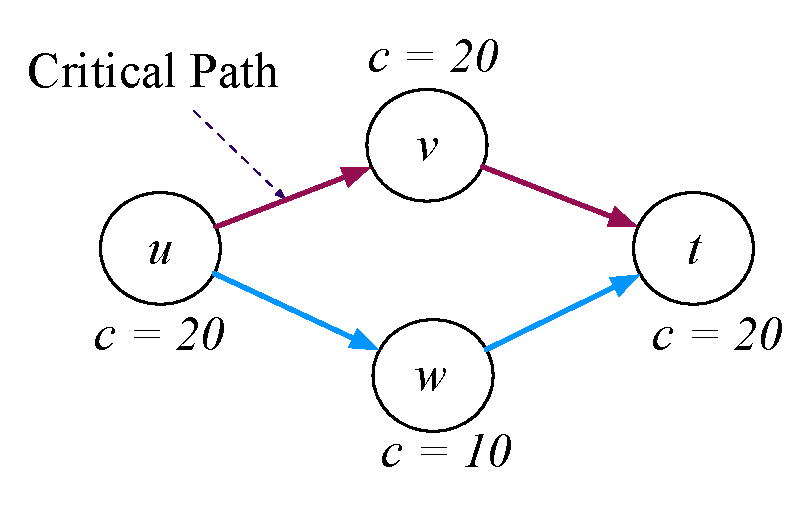
\includegraphics[width=0.4\columnwidth]{dag}
  \caption{An Example of a Parallel Real-time Task}
  \label{fig:dag}
\end{figure}

\revise{A node $v_i^j \in V_i$ is expressed as a double <$cs_i^j$, $c_i^j$>, where $cs_i^j$ denotes the code segment executed by a thread and $c_i^j$ denotes the worst-case execution time of the thread execution.}
Each node ${v \in V_i}$ of a DAG ${G_i = (V_i, E_i)}$ represents the
execution of a thread and an ${e \in E_i}$ edge represents a
dependency between two nodes. A dependency between two nodes indicates
that a node is ready to execute only upon the completion of all its
predecessor nodes. We consider a source as a node with no incoming
arcs and a sink as node with no outgoing arcs. For the sake of
simplicity, we assume a task has only one source and sink node. In
practice, this not hard to achieve as a source and sink can be added
to the task with $0$ execution and not change the task dependencies.

%Nodes of a task have an associated worst-case execution time. 
\revise{For a node $v_i^j$, we define $parent(v_i^j)$ and $child(v_i^j)$ as a set of parent nodes of $v_i^j$ and a set of child nodes of $v_i^j$, respectively. we define $pre(v_i^j)$ and $succ(v_i^j)$ as a set of all predecessors of $v_i^j$ and a set of all successors of $v_i^j$, respectively.}
For any given task, we define a \textit{critical path} $\lambda_i$ of a 
task $\tau_i$ as the longest execution time path that starts from
source and ends at the sink. \textit{Critical path length} ($L_i$) is
defined as the sum of execution times of all nodes along the critical
path $\lambda_i$ of task $\tau_i$.  Workload $C_i$ of
a task $\tau_i$ is defined as the sum of worst-case execution time of
all nodes in the DAG task. 


\subsection{Federated Scheduler}
For a task set $\tau$ , the federated scheduling algorithm works as
follows. We first divide the task sets into two disjoint sets
$\tau_{high}$  and $\tau_{low}$. $\tau_{high}$ contains all tasks with
high utilization (i.e. $u_i > 1$) and $\tau_{low}$ contains all
remaining low utilization tasks. Each task in $\tau_{high}$ is
assigned $m_i$ dedicated cores (no other task is executed on these
cores), where: \begin{equation}\label{eq:m} m_i = \left\lceil \frac{C_i - L_i}{D_i - L_i}
\right\rceil \end{equation}

We use $m_{high} = \sum_{\tau_i \in \tau_{high}} m_i$ to denote the total
number of cores assigned to high-utilization tasks. We assign
the remaining cores to all low-utilization tasks $\tau_{low}$, denoted
as ${m_{low} = m - m_{high}}$. The federated scheduling algorithm admits
the task set ${\tau}$, if $m_{low}$ is non-negative and all tasks in
$\tau_{low}$ are schedulable sequentially.  

After a valid core allocation, runtime scheduling proceeds as
follows. Any greedy (work-conserving) parallel scheduler can be used
to schedule a high-utilization task $\tau_i \in \tau_{high}$ on its
assigned $m_i$ cores. Informally, a greedy scheduler is one that never
keeps a core idle if some node is ready to execute. 

All low-utilization tasks are treated and executed as though they are
sequential tasks and any multiprocessor scheduling algorithm (such as
partitioned EDF, or various rate-monotonic schedulers) can be used to
schedule all the low-utilization tasks on the allocated $m_{low}$
cores. We can safely treat low-utilization tasks as sequential tasks
since $C_i \le D_i$ and parallel execution is not required to meet their
deadlines. 

\subsection{Processing Model}

In this work, for each core, we assume a dedicated direct mapped
instruction cache. We assume a time-compositional architecture\addcite,
where memory and execution demand are separable. Copying a block of 
main memory to cache memory requires ${\mathbb{B}}$ cycles, commonly
referred to as the the block reload time (BRT). If multiple cores share
the same processing platform their cache contents do not interfere with
one another. The impact of a shared cache between cores is not considered.


\section{Proposed Changes to the Directed Acyclic Graph Model of Parallel Systems}

For a DAG ${G = (V, E)}$ representing a parallel task, each node ${v_i \in V}$ represents
the release, execution, and termination of a single thread within one task 
\addcite. In the existing model, the only relationship between thread releases and the executable object they execute is the worst-case execution time of the node. Two nodes ${v_i, v_j \in V}$ may represent two threads executing the same object (possibly on different processors).

\begin{figure}
  \centering
  \begin{subfigure}[b]{0.4\textwidth}{
      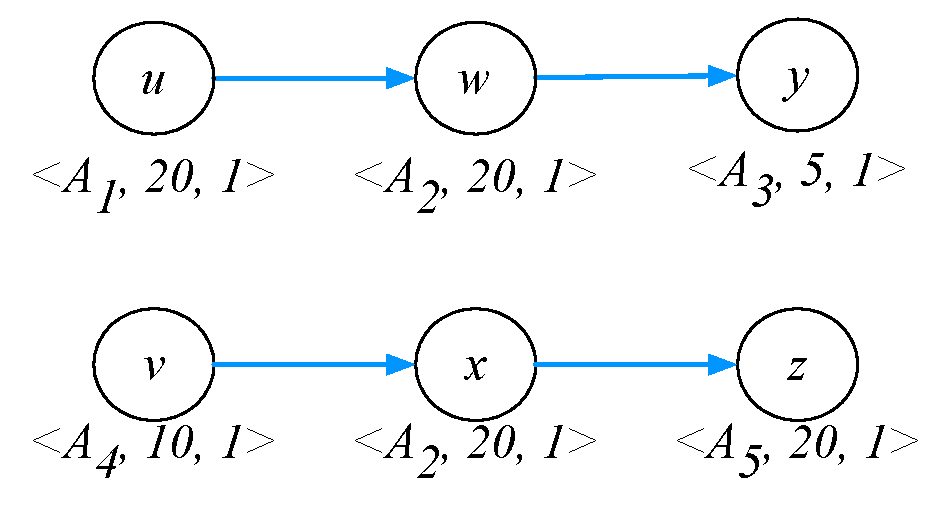
\includegraphics[width=\textwidth]{beforeCollapse}
      \caption{Before Collapse}
      \label{fig:before-collapse}
    }
  \end{subfigure} \quad
  \begin{subfigure}[b]{0.4\textwidth}{
      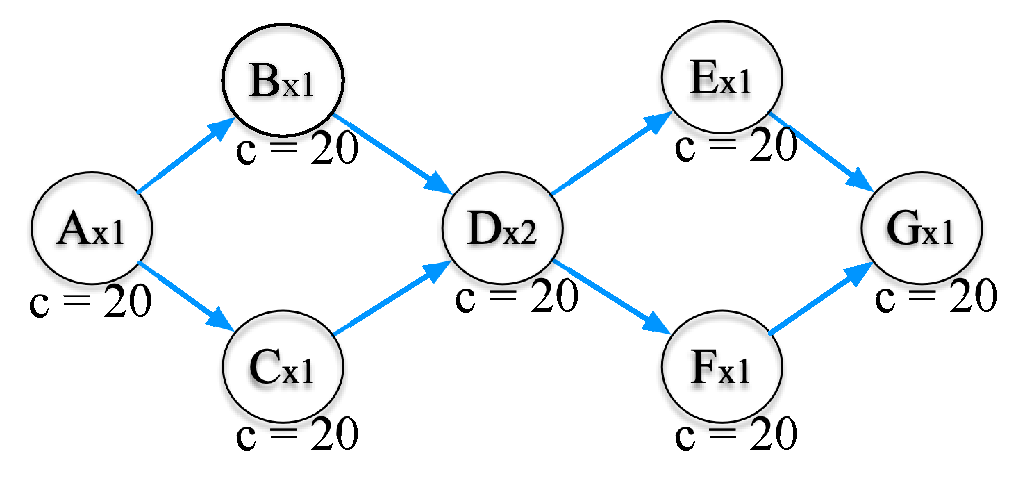
\includegraphics[width=\textwidth]{afterCollapse}
      \caption{After Collapse}
      \label{fig:after-collapse}
    }
  \end{subfigure}
  \caption{DAG Node Change from Thread to Code Segment}
  \label{fig:dag-change}
\end{figure}

To take advantage of instruction cache reuse, we propose a simple modification to the DAG
model. Where possible, distinct nodes that represent the execution of
the same object are collapsed into a single node. To accommodate collapse,
nodes are identified by their executable object, and a new attribute is added to every node
indicating the number of threads which will be executed over the object.

\revise{Given the new model to represent a node, two nodes $v_i^j$, $v_i^k$ with the same code segments (i.e., $cs_i^j = cs_i^k$ and $c_i^j = c_i^k$) are collapsed into one node $v_i^h$, where $v_i^h = <cs_i^j, c_i^j, \max{\eta_i^j, \eta_i^k}+1>$.  To ensure dependencies of the DAG are not violated, we replace the edges that start from $v_i^j$ and $v_i^k$  to start from $v_i^h$, i.e., the child nodes of $v_i^h$ are given as a union of the child nodes of $v_i^j$ and $v_i^k$, $child(v_i^h) = child(v_i^j) \cup child(v_i^k)$. Similarly, parent nodes of $v_i^h$ are given as a union of the parent nodes of $v_i^j$ and $v_i^k$, i.e., $parent(v_i^h) = parent(v_i^j) \cup parent(v_i^k)$.}

Figure~\ref{fig:dag-change} illustrates the proposed change. Nodes in
Figure~\ref{fig:before-collapse} are labeled with the code segment
they are associated with. Two nodes of ${B}$ are collapsed in
Figure~\ref{fig:after-collapse}, where each node is attributed with
the number of threads executed over the code segment.

A goal of this work is to bring the inter-thread cache benefit \addcite to parallel DAG tasks. 

%% ct - commented out because splitting a code segment into multiple code segments may introduce loops in the DAG. 
%%		For example, if a loop is too big and cannot fit into a cache block then we it will be split across multiple segments which will introduce a DAG.
%%
%%A goal of this work is to bring the inter-thread cache benefit \addcite to parallel DAG tasks. As a first-step, two requirements are placed on nodes of the graph.
%%\begin{description}
%%\item[R1] All executable objects must fit entirely within the cache.
%%\item[R2] No two instructions of an executable object may evict one another.
%%\end{description}
%%
%%Requirements R1 and R2 may be met for any executable object by repeatedly dividing
%%the object source that result in objects larger than the cache into separate code segments, carefully recompiling those code segments to maximize cache use, and replacing the original node with a serial set of nodes.
%%\\
%%\\
%%\emph{ct-3 A figure is needed to illustrate the transformation from one over-sized node, to multiple correctly sized nodes}
%%\\

In the established model \addcite, each node ${v_i^j \in V_i}$ is characterized
with a single worst case execution time for a single thread. We
propose that each node's WCET is characterized by a function
${c_i^j(\eta_i^j)}$ where ${\eta_i^j}$ is the number of threads that will execute the
node ${v_i^j}$ on the same core serially (one after another) with no
other thread executing a different object on the core in between executions.

%%Given a timing-compositional architecture with the restrictions \textbf{R1} and \textbf{R2},
Given a timing-compositional architecture
${c_i(n)}$ can be expressed for any node in terms of the memory demand of all instructions
of ${v_j \in V_i}$ into the cache ${\gamma_j}$ and the worst-case execution demand
to execute the node assuming all instructions of ${v_j}$ have
been cached ${\iota_j}$. Equation~\ref{eq:c_i} is an expression for
${c_i(n)}$. 
 
\begin{equation}
  \label{eq:c_i}
  c_i(n) = \begin{cases}
    0, & n \le 0 \\
    \gamma_j + \iota_j \cdot n, & n > 0
  \end{cases}
\end{equation}

For a node ${v_i \in V_j}$, the upper bound of memory demand of the node is denoted ${\gamma_i}$. It is the number of cycles required to load all blocks of the node. The complete set of blocks of the node are equivalent to the evicting cache blocks (ECBs)\addcite [Tan \& Mooney] of the object. Thus, the memory demand is the product of the BRT and count of ECBs of the node ${\textsc{ecb}_i}$ found in Equation~\ref{eq:mem-demand}.

\begin{equation}{\label{eq:mem-demand}}
    \gamma_i = \mathbb{B} \cdot \textsc{ecb}_i
\end{equation}

The execution demand ${\iota_i}$ for a node ${v_i^j \in V_i}$ is the worst case execution time of a single thread given all instructions are present in the cache. Any suitable WCET calculation method {\addcite} may be used to calculate the value.

%%\section{Problem Formulation}

\section{Node Collapse}

\revise{Given the new model to represent a node, two nodes $v_i^j$, $v_i^k$ with the same code segments (i.e., $cs_i^j = cs_i^k$ and $c_i^j = c_i^k$) are collapsed into one node $v_i^h$, where $v_i^h = <cs_i^j, c_i^j, \max{\eta_i^j, \eta_i^k}+1>$.  To ensure dependencies of the DAG are not violated, we replace the edges that start from $v_i^j$ and $v_i^k$  to start from $v_i^h$, i.e., the child nodes of $v_i^h$ are given as a union of the child nodes of $v_i^j$ and $v_i^k$, $child(v_i^h) = child(v_i^j) \cup child(v_i^k)$. Similarly, parent nodes of $v_i^h$ are given as a union of the parent nodes of $v_i^j$ and $v_i^k$, i.e., $parent(v_i^h) = parent(v_i^j) \cup parent(v_i^k)$.}

\begin{figure}
  \centering
  \begin{subfigure}[b]{0.4\textwidth}{
      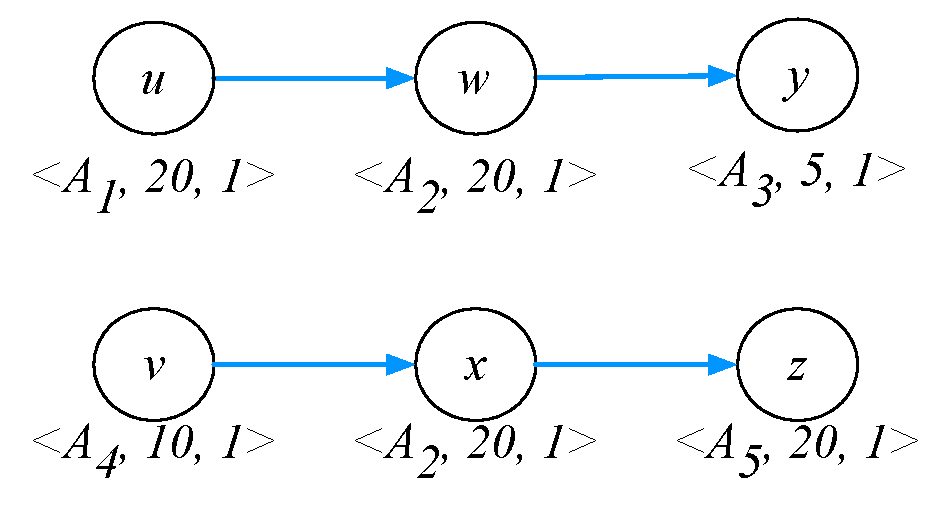
\includegraphics[width=\textwidth]{beforeCollapse}
      \caption{Before Collapse}
      \label{fig:before-collapse}
    }
  \end{subfigure} \quad
  \begin{subfigure}[b]{0.4\textwidth}{
      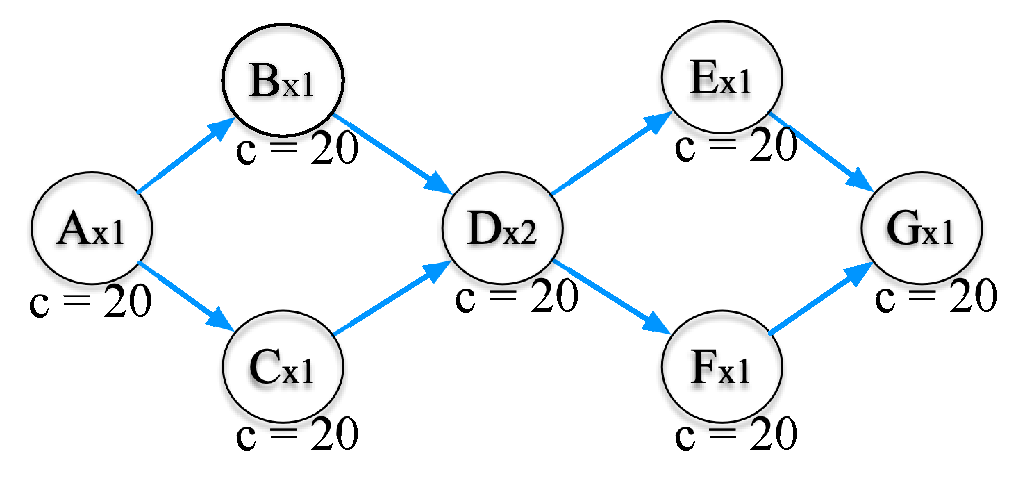
\includegraphics[width=\textwidth]{afterCollapse}
      \caption{After Collapse}
      \label{fig:after-collapse}
    }
  \end{subfigure}
  \caption{DAG Node Change from Thread to Code Segment}
  \label{fig:dag-collapse}
\end{figure}


\revise{A property of collapse must be stated. When collapsing two
  nodes ${u,v \in V}$ if one node is on the critical path (call it
  ${u}$) but the other is not (${y}$), then collapse must assign
  threads of ${y}$ to ${u}$.}

\revise{A property of collapse must be stated. When collapsing two
  nodes ${u,v \in V}$ to one node ${u}$ the length of the critical
  path is reduced by the WCET of ${v}$ before collapse and increased
  by the WCET of ${u}$ after collapse}
  


Figure~\ref{fig:dag-collapse} illustrates the proposed change. Nodes in
Figure~\ref{fig:before-collapse} are labeled with the code segment
they are associated with. Two nodes of ${B}$ are collapsed in
Figure~\ref{fig:after-collapse}, where each node is attributed with
the number of threads executed over the code segment.


\section{Candidacy for collapse}

\subsection{Conditions for Candidacy of Collapse}
For a task ${\task{i} \in \tasks{}}$, associated DAG ${\Dag{i}
  \in \dagset{}}$, where ${\Dag{i} = (V, E)}$,
the nodes ${u,v \in V}$ qualify as \emph{candidates} for collapse if
and only if the following conditions are true:
\begin{enumerate}
  \item Nodes ${u}$ and ${v}$ refer to execution of the same object.
  \item Collapsing ${u}$ and ${v}$ cannot not introduce a cycle in ${G_i}$.
  \item The sum of the individual worst-case execution times of ${u}$
    and ${v}$ is greater than the collapsed worst-case execution time
    of ${u}$ and ${v}$ i.e. ${c(u) + c(v) > c(u + v)}$.
\end{enumerate}

\revise{Following paragraph should state: One property of collapse is
  that loops cannot be introduced for two nodes to remain candidates
  of collapse.
}
In a DAG ${G_i = (V_i, E_i)}$, collapsing two nodes that represent the
execution of the same code segment may result in a violation of the
DAG. For example, Fig~\ref{fig:dag-violation} shows one such example
where collapsing two nodes with the same code segment $B$ results in a
loop inside the DAG. In this section, we derive the necessary and
sufficient condition for a pair of nodes when satisfied does not
result in a DAG violation after a collapse.

\revise{Needed: introductory paragraph to state the following theorem
  provides a condition for ensuring collapse does not introduce loops}

\begin{figure}
  \centering
  \begin{subfigure}[b]{0.48\textwidth}{
      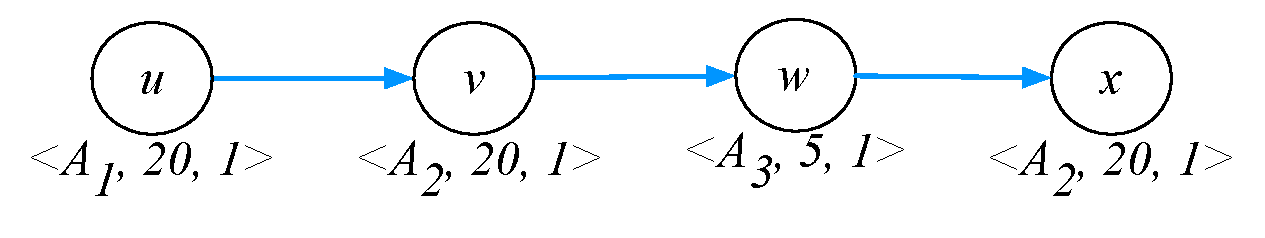
\includegraphics[width=\textwidth]{beforeViolation}
      \caption{Before Collapse}
      \label{fig:beforeViolation}
    }
  \end{subfigure}~
  \begin{subfigure}[b]{0.33\textwidth}{
      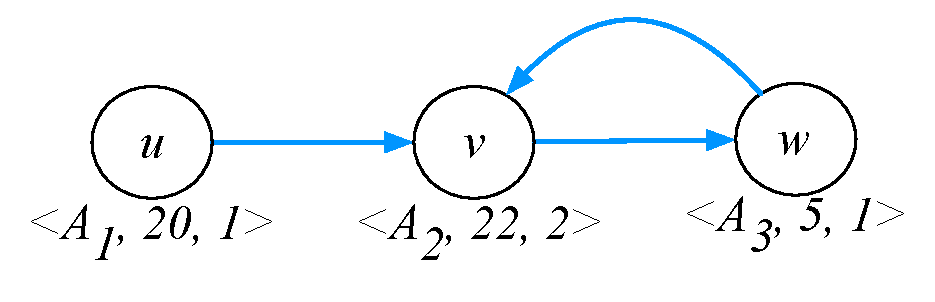
\includegraphics[width=\textwidth]{afterViolation}
      \caption{After Collapse}
      \label{fig:afterViolation}
    }
  \end{subfigure}
  \caption{Collapse of two nodes can result in a loop inside the DAG task}
  \label{fig:dag-violation}
\end{figure}

\revise{expand both definitions} \\
\textbf{Definition ${u \prec v}$} -- indicates that ${u}$ appears
before ${v}$ in a topological sort of ${G}$. \\
\textbf{Definition ${d(u, v)}$} -- is the greatest number of edges
along a directed path from ${u}$ to ${v}$ in ${G}$. When no path
exists, ${d(u,v) = 0}$.

\begin{theorem}[Candidacy for Collapse]
  For a DAG ${G = (V, E)}$ and nodes ${u, v \in V}$ where ${u \prec
    v}$, ${u}$ and ${v}$ can be collapsed without introducing a loop
  if and  only if ${d(u, v) \le 1}$.
\end{theorem}


\begin{theorem}[Candidacy for collapse] \label{thrm:candidacy-collapse} Two nodes $v_i^j$ and $v_i^k$ in a DAG task $\tau_i$ when collapsed do not introduce a loop if and only if $d(v_i^j, v_i^k) \le 1$ and $d(v_i^k, v_i^j) \le 1$, where $d(v_i^j, v_i^k)$ is the length of the longest path between $v_i^j$ and $v_i^k$ as obtained by depth first search. \end{theorem}
\begin{proof}
%The proof is divided into two parts
We divide the proof into two parts. We first prove that the condition $d(v_i^j, v_i^k) \le 1$ and $d(v_i^k, v_i^j) \le 1$ is a necessary condition for candidacy and latter we prove that the condition is a sufficient condition.

%First part - necessary part - to prove that if the constraint is violated then it will result a violation of the dag 
If the condition is not satisfied $d(v_i^j, v_i^k) \le 1$ and $d(v_i^k, v_i^j) \le 1$, then it implies that there is a path from $v_i^j$ to $v_i^k$ or a path from $v_i^k$ and $v_i^j$ with length greater than 1, i.e., $\exists p1 \  such \  that p1 = {v_i^j, v_i^l, \cdots , v_i^k} or p1 = {v_i^k, v_i^l, \cdots , v_i^l}$. When nodes $v_i^j$ and $v_i^k$ are collapsed into $v_i^h$, $p1$ will be modified to ${v_i^h, v_i^l, \cdots , v_i^h}$ which forms a loop. 

%Second part -  sufficient part - if the constraint is met there is no other source of a loop
To prove the sufficient condition, we first prove the contra-positive to be true, i.e., a DAG violation occurs only when the condition $d(v_i^j, v_i^k) \le 1$ and $d(v_i^k, v_i^j) \le 1$ is true. A DAG violation in the collapsed DAG implies that there exists a path $p1$ in the collapsed DAG given by $v_i^h, v_i^l, \cdots , v_i^h$ with a length greater than or equal to 2.  Since there are no loops in the original DAG, only a collapsed node can cause a loop in the collapsed DAG. Therefore, $v_i^h$ should be the collapsed node. In the original DAG, one node of $v_i^h$ corresponds to $v_i^j$ and the other node corresponds to $v_i^k$. In the original DAG, $p1$ must correspond to ${v_i^j, v_i^l, \cdots , v_i^k} or {v_i^k, v_i^l, \cdots , v_i^l}$. Thus, a DAG violation in the collapsed DAG implies that there exists a path from $v_i^j$ to $v_i^k$  or $v_i^k$ and $v_i^j$ with a length greater than or equal to 2. 

Therefore, we can conclude that two nodes $v_i^j$ and $v_i^k$ in a DAG task $\tau_i$ when collapsed do not introduce a loop if and only if $d(v_i^j, v_i^k) \le 1$ and $d(v_i^k, v_i^j) \le 1$.
\end{proof}

In summary, we define two nodes $v_i^j$ and $v_i^k$ to be {\textbf candidates for collapse} if they have the same code block and $d(v_i^j, v_i^k) \le 1$ and $d(v_i^k, v_i^j) \le 1$, where $d(v_i^j, v_i^k)$ is the length of the longest path between $v_i^j$ and $v_i^k$.


%
% XXX-ct Remove the proposed directory and tex files, they remain for
% instructive purposes only
%
% \section{Proposed Method - For High Utilization Tasks}
\revise{We define candidates for collapse as a pair of nodes that share the same cache block, and other conditions. Identifying potential candidates for collapse is discussed in the following/previous section. For this section, we assume that the potential candidates are at the same depth from the start node and they are not dependent on each other. } 

In a federated scheduler, a high utilization task $T_i$ is allocated $m_i$ dedicated cores, given by Equation (\ref{eq:m}), where no other tasks can execute. In this environment, collapsing two nodes in the DAG of high utilization task $T_i$ is beneficial to the federated scheduler if the collapse decreases the required number of cores. Formally, consider the number of cores dedicated to a task ${T_i}$ before any two nodes are collapsed as ${m_i}$ as calculated by Equation~\ref{eq:m}. The number of cores dedicated to ${T_i}$ after collapse are denoted ${\hat{m}_i}$.

\textbf{Beneficial Collapse}: Collapsing two nodes of a task ${T_i}$ is \emph{beneficial} if ${\hat{m}_i \le m_i}$.

\revise{We need more supportive definitions before the proof, \\ 
  1 inter-thread cache benefit for two collapsed nodes ${v_j}$ and ${v_k}$ for the same executable object \\
  2 max extension of paths by ${\iota_j}$ for two collapsed nodes ${v_j}$ and ${v_k}$. \\
  3 "resulting path" -- the single path that results from ${v_j}$ and ${v_k}$ being collapsed from separate paths
  }

In Theorem~\ref{thrm:conditional-collapse}, we derive a sufficient condition to determine if collapsing two nodes is beneficial. The proof is divided into four sections. Each is related to the impact of collapse upon the longest path through the DAG of ${T_i}$.

%\newtheorem{theorem}{Theorem}
\begin{theorem}[Conditional Collapse]\label{thrm:conditional-collapse} For a DAG task ${\tau_i}$, collapsing two \textbf{candidate} nodes ${v_j, v_k \in V_i}$ (which refer to the same executable object) is \textbf{beneficial} if:

    \begin{equation}\label{eq:cond}
        1 + \frac{\gamma_j}{\iota_j} > \frac{C_i  - L_i }{D_i - L_i}
    \end{equation}
\end{theorem}
\begin{proof}
A direct proof supports the theorem, it is divided into four cases 1.) collapsing two nodes off the critical path where the critical path length is not affected 2.) collapsing two nodes with exactly one lies on the critical path 3.) collapsing two nodes where both lie on the critical path 4.) collapsing two nodes off the critical path, which creates a new critical path length.

\emph{Case 1.} Collapsing two nodes off the critical path with no impact to the critical path length. Since ${v_j}$ and ${v_k}$ refer to the same executable object ${\iota_j = \iota_k}$ and ${\gamma_j = \gamma_k}$. Collapsing ${v_j}$ and ${v_k}$ in the graph serializes the execution of threads on the same processor. This decreases the execution time ${v_k}$ (or ${v_j}$) due to the inter-thread cache benefit; which is quantified as ${2 \cdot \iota_j + \gamma_j}$. This increases the path(s) of ${v_j}$ and ${v_k}$ by at most ${\iota_j}$. 
\end{proof}
%\end{theorem}
%\blacksquare

Collapsing two nodes of DAG tasks always results in a decrease in the worst-case execution time of the task by $\mathbb{B}$. Nevertheless, collapsing two nodes of DAG tasks may increase the critical path by $\mathbb{I}$, may increase the critical path by a value less than $\mathbb{I}$ but greater than $0$, or may not change the critical path length value. For example, Fig.~\ref{fig:c1}, Fig~\ref{fig:c2}, and Fig.~\ref{fig:c3} show the three cases, i.e., case 1 when there is no change in critical path length, case 2 when the critical path length increases by $\mathbb{I}$, and case 3 when the critical path length increases by a values greater than $0$ but less than $\mathbb{I}$.

\begin{figure}
  \centering
  \begin{subfigure}[b]{0.4\textwidth}{
      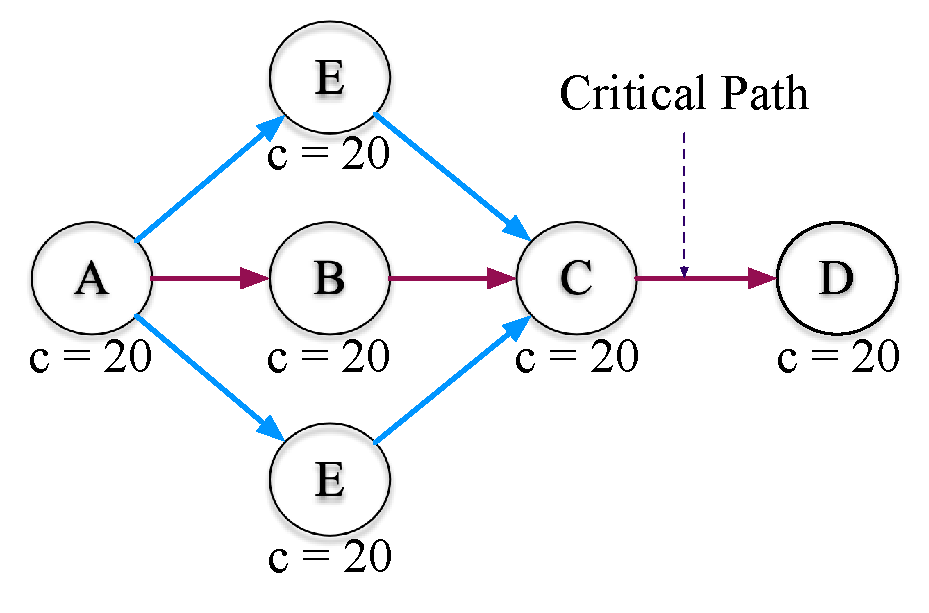
\includegraphics[width=\textwidth]{c1before}
      \caption{Before Collapse}
      \label{fig:c1before}
    }
  \end{subfigure}~
  \begin{subfigure}[b]{0.4\textwidth}{
      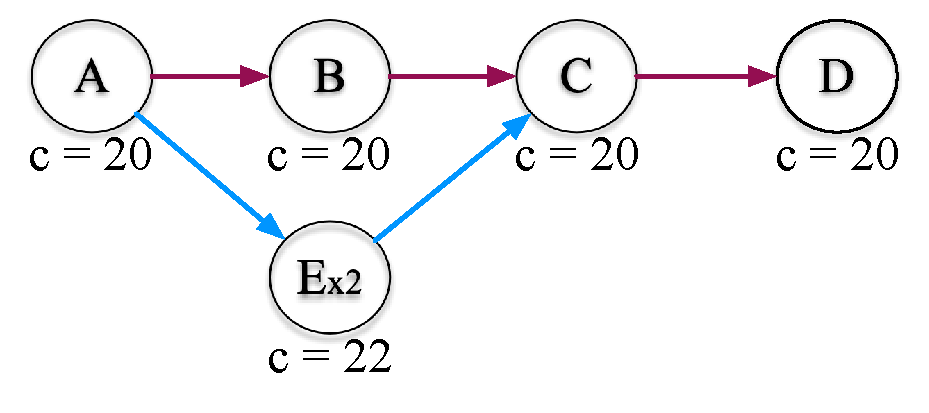
\includegraphics[width=\textwidth]{c1after}
      \caption{After Collapse}
      \label{fig:c1after}
    }
  \end{subfigure}
  \caption{Case 1:  No change in the critical path length}
  \label{fig:c1}
\end{figure}

\begin{figure}
  \centering
  \begin{subfigure}[b]{0.4\textwidth}{
      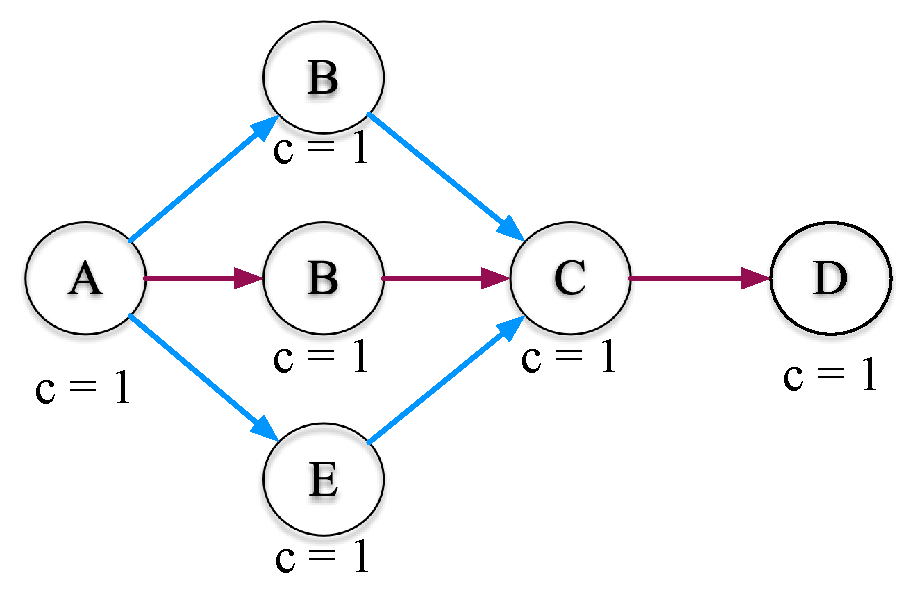
\includegraphics[width=\textwidth]{c2before}
      \caption{Before Collapse}
      \label{fig:c2before}
    }
  \end{subfigure}~
  \begin{subfigure}[b]{0.4\textwidth}{
      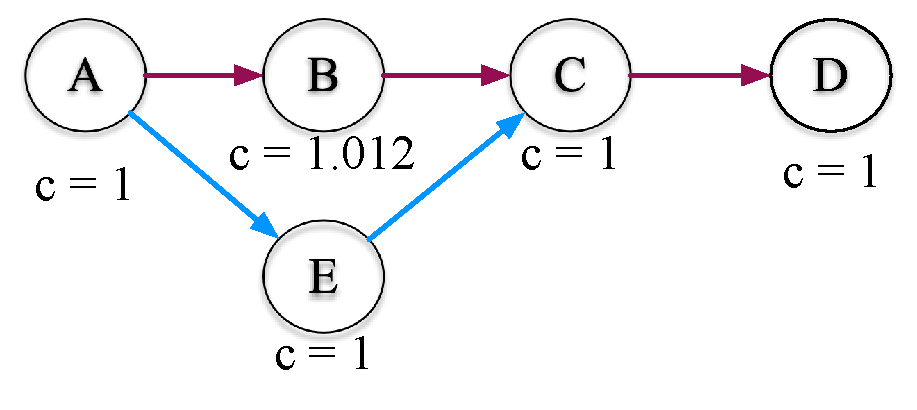
\includegraphics[width=\textwidth]{c2after}
      \caption{After Collapse}
      \label{fig:c2after}
    }
  \end{subfigure}
  \caption{Case 2:  Critical path length increases by $\mathbb{I}$}
  \label{fig:c2}
\end{figure}

\begin{figure}
  \centering
  \begin{subfigure}[b]{0.4\textwidth}{
      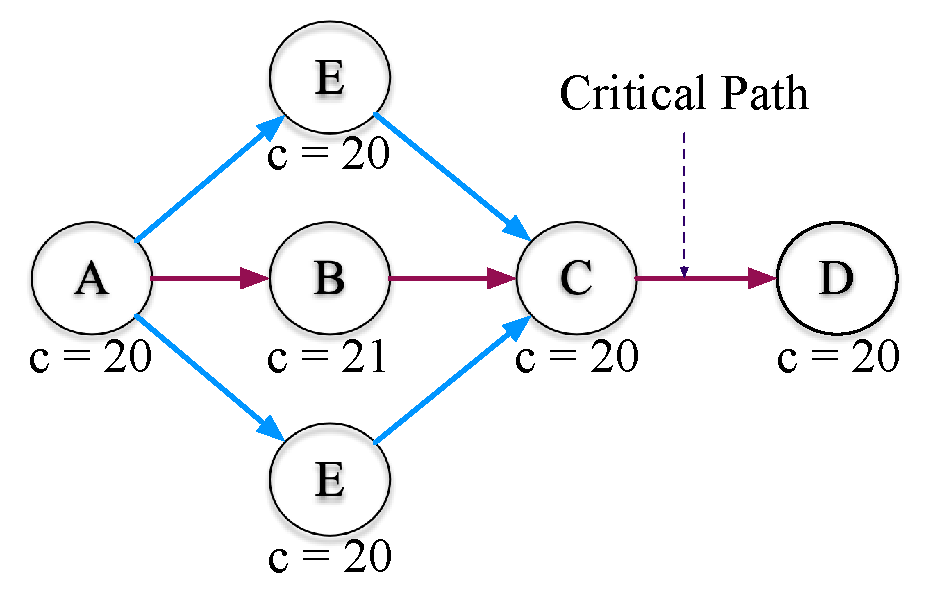
\includegraphics[width=\textwidth]{c3before}
      \caption{Before Collapse}
      \label{fig:c2before}
    }
  \end{subfigure}~
  \begin{subfigure}[b]{0.4\textwidth}{
      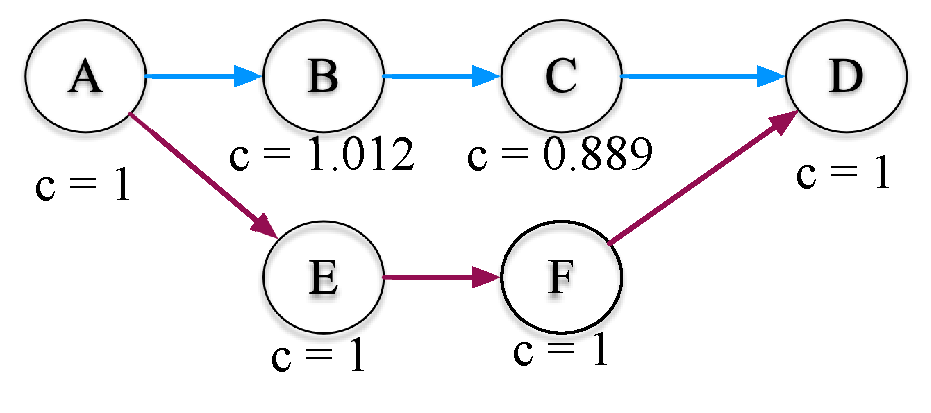
\includegraphics[width=\textwidth]{c3after}
      \caption{After Collapse}
      \label{fig:c2after}
    }
  \end{subfigure}
  \caption{Case 3:  Critical path length increases by a value less than $\mathbb{I}$}
  \label{fig:c3}
\end{figure}

In case 1, there is no change in the critical path length but the worst case execution decreases by $\mathbb{B}$,thus the required number of cores after collapse, given by $\frac{C_i - \mathbb{B} - L_i}{D_i - L_i}$, is less than the required number of cores before collapse, given by $\frac{C_i - L_i}{D_i - L_i}$  (since $\frac{C_i - \mathbb{B} - L_i}{D_i - L_i} < \frac{C_i - L_i}{D_i - L_i}$). Therefore, any two nodes that fall under case 1 can be considered for collapse. 

In case 2, the task $T_i$ saves $\mathbb{B}$ units of worst-case execution time however it increases the critical path length by $\mathbb{I}$. Similarly, in case 3, the task $T_i$ saves $\mathbb{B}$ units of worst-case execution time however it increases the critical path length by at most $\mathbb{I}$. To derive a sufficient condition, we consider the upper bound on the increase in critical path length, i.e., $\mathbb{I}$ as the increase in critical path length. Thus, under case 2 and 3, a task receives a saving of $\mathbb{B}$ in worst-case execution time but spends $\mathbb{I}$ on the critical path. In case 2 and 3, collapsing two nodes can decrease the number of cores if Equation (\ref{eq:cond}) holds.

\begin{equation} \label{eq:cond} 1 + \frac{\mathbb{B}}{\mathbb{I}} > \frac{C_i  - L_i }{D_i - L_i} \end{equation}

To prove this, let us assume the Equation (\ref{eq:inequality}) is true.
\begin{equation} \label{eq:inequality} \frac{C_i - \mathbb{B} - (L_i + \mathbb{I})}{D - (L_i + \mathbb{I})}  < \frac{C_i  - L_i }{D_i - L_i} \end{equation}
Then by algebraic simplification, the following inequality is also true.
$$ - ( \mathbb{B} + \mathbb{I}) (D_i - L_i)  < -\mathbb{I}(C_i  - L_i )$$
Further simplification shows that the following inequality is also true.
$$ 1 + \frac{\mathbb{B}}{\mathbb{I}} > \frac{C_i  - L_i }{D_i - L_i}$$
Since the obtain result is obtained from algebraic simplification of Equation (ref{eq:inequality}), we can conclude that if Equation (\ref{eq:cond}) is true then Equation (\ref{eq:inequality}) is also true.

% Section cbound \ref{sec:collapse-bound}
%   Contains proof of the change in ${m}$ when collapsing candidate
%   nodes.
\section{Collapsing of Nodes}
\label{sec:collapse-bound}

For a task ${\task{i} \in \tasks{}}$, associated DAG
${\Dag{i} \in \dagset{}}$, where ${\Dag{i} = (V, E)}$, with nodes
${u,v \in V}$ that qualify as candidates for collapse, collapsing
${u}$ and ${v}$ may (or may not) result an increase in
performance. This section is provides a method of determining if the
collapse of ${u}$ and ${v}$ will \emph{benefit} performance of the
task set ${\tasks{}}$ in terms of ${m_i}$: the number of cores
dedicated to \task{i}.

For a task \task{i} with \noofcores{i} dedicated cores, collapsing
${u}$ and ${v}$ benefits \task{i} (and therefor \tasks{}) if the
number of cores dedicated to \task{i} is potentially reduced. If
\noofcores{i} is the number of cores dedicated to \task{i} before
collapsing ${u}$ and ${v}$, and ${\hat{\noofcores{i}}}$ the number of
cores after collapse, beneficial collapse is defined as follows: 

\begin{definition}[Beneficial Collapse]
  Collapsing ${u}$ and ${v}$ is \emph{beneficial} if and only if
  ${\hat{\noofcores{i}} \le \noofcores{i}}$.
\end{definition}

The number of cores dedicated to task \task{i} is determined by
Equation~\ref{eq:m} which is replicated below. Equation~\ref{eq:m}
depends on the critical path length \criticalpathlen{i} and workload
\workload{i}, both of which can be affected by collapsing nodes.

\begin{multicols}{2}
  \begin{equation*}
    m_i = \left\lceil
      \frac{\workload{i} - \criticalpathlen{i}}
           {\Deadline{i} - \criticalpathlen{i}}
    \right\rceil
  \end{equation*}
  \begin{equation*}
    \workload{i} = \sum_{v \in V} c_v(\eta_v)
  \end{equation*}
\end{multicols}

For simplicity of presentation, it is assumed the entire object each
thread assigned to ${v}$ executes fits entirely within the
cache of each core. Additionally, each core is required to be
timing-compositional~\addcite{}, where the memory and execution demand
are separable. The memory demand of populating the cache with the
entire object ${\alpha_v}$ associated with ${v}$ is referred to as
${\mathbb{B}_v}$. Execution demand of one thread over ${\alpha_v}$ is
referred to as ${\mathbb{I}_v}$. 

Applying the principle of inter-thread cache benefit from \addcite{}
[BUNDLE and BUNDLEP], the WCET of a node ${v}$ is given by:

\begin{equation}
  c_v(\eta_v) = \mathbb{B}_v + \eta_v \cdot \mathbb{I}_v
\end{equation}

When comparing parameters before and after collapse, the after
collapse values will be give a ``hat'' indicator. For example, the
critical path length before collapse is denoted
\criticalpathlen{i}; after collapse it is denoted
${\hat{\criticalpathlen{i}}}$.

When two nodes ${u,v \in V}$ are collapsed into ${\hat{u}}$, the WCET
of ${\hat{u}}$ can be described in terms of the WCET of ${u}$ and
${v}$. Under the assumption that ${\alpha_u}$ fits entirely in the
cache, combined with the timing-compositional 
requirement of each core, scheduling ${\eta_u}$ followed by ${\eta_v}$
threads on the same core places all values in the cache before they
are executed. Therefor, the memory demand of ${\eta_u + \eta_v}$
threads is ${\mathbb{B}_u}$. The separable execution demand of
${\eta_u}$ followed by ${\eta_v}$ threads is ${(\eta_u + \eta_v) \cdot
  \mathbb{I}_u}$ because ${\mathbb{I}_u = \mathbb{I}_v}$. Thus, the
WCET of ${\hat{c}_u(u)}$ can be defined as  
follows:
\begin{equation*}
  \hat{c}_u(u) = c_u(u + v) = \mathbb{B}_u + (\eta_u + \eta_v) \cdot
      \mathbb{I}_u 
\end{equation*}

\begin{theorem}[Conditional Collapse] For a task
  ${\task{i} \in \tasks{}}$, associated DAG ${\Dag{i} \in \dagset}$,
  where ${\Dag{i} = (V, E)}$, candidate nodes ${u,v \in V}$,
  collapsing ${u}$ and ${v}$ into ${\hat{u}}$ is beneficial if:

  \begin{equation}
    \indent
    1 + \frac{\mathbb{B}_u}{\eta_v \cdot \mathbb{I}_u}
    \ge
    \frac{\workload{i} - \criticalpathlen{i}}
         {\Deadline{i} - \criticalpathlen{i}}
    \label{eq:condition}
  \end{equation}

  \begin{proof}
    The goal of the proof is to show the comparison of
    Equation~\ref{eq:collapse-condition} is true
    under all circumstances. There are four cases which cover all
    possible changes to the critical path length and workload of the
    task \task{i}. Note, the deadline of the task \Deadline{i} cannot
    be changed and does not need consideration. 

    \begin{equation} \label{eq:collapse-condition}
      \indent
      \frac{\hat{\workload{i}} - \hat{\criticalpathlen{i}}}
           {\Deadline{i} - \hat{\criticalpathlen{i}}} \le
      \frac{\workload{i} - \criticalpathlen{i}}
           {\Deadline{i} - \criticalpathlen{i}}
    \end{equation}

    In summary, the four cases to consider are:

    \begin{enumerate}
    \item ${(u, v \not \in \criticalpath{i})
      \land
      (\hat{u} \not \in \hat{\criticalpath{i}})}$:
      Neither node is on the critical path before collapse and
      ${\hat{u}}$ is not on the critical path after collapse. 
    \item ${(u \in \criticalpath{i} \land v \not \in \criticalpath{i})
      \land
      (\hat{u} \in \hat{\criticalpath{i}})}$: One node (call it ${u}$)
      is on the critical path before collapse and remains on the path
      after collapse.
    \item ${(u,v \in \criticalpath{i}) \land
      (\hat{u} \in \hat{\criticalpath{i}})}$: Both nodes lie
      on the critical path before collapse.
    \item ${(u,v \not \in \criticalpath{i}) \land
      (\hat{u} \in \hat{\criticalpath{i}})}$: Neither node
      belongs to the critical path before collapse. Collapsing the
      nodes creates a \textbf{new} critical path.
    \end{enumerate}

    \begin{case}[${(u, v \not \in \criticalpath{i}) \land
          (\hat{u} \not \in \hat{\criticalpath{i}})}$] By
      definition of critical path and critical path length, ${u}$ and
      ${v}$ do not contribute to \criticalpathlen{i} nor ${\hat{u}}$ to
      ${\hat{\criticalpathlen{i}}}$. Therefor,
      ${\criticalpathlen{i} = \hat{\criticalpathlen{i}}}$. The
      workload has been affected by the removal of ${v}$ and ${u}$'s execution
      and the increase in ${\hat{u}}$'s execution. 
      \begin{align}
        \indent
        \hat{C}_i &= C_i - c_u(\eta_u) - c_v(\eta_v) +
        \hat{c}_u(\eta_u + \eta_v) \\
        &= C_i - \mathbb{B}_u - \eta_u \cdot \mathbb{I}_u
            - \mathbb{B}_v - \eta_v \cdot \mathbb{I}_v +
            \hat{c}_u(\eta_u + \eta_v)
            \label{eq:pre-u} \\
        &= C_i - \mathbb{B}_u - \eta_u \cdot \mathbb{I}_u
            - \mathbb{B}_u - \eta_v \cdot \mathbb{I}_u +
            \hat{c}_u(\eta_u + \eta_v)
            \label{eq:post-u} \\
        &= C_i -2\mathbb{B}_u - (\eta_u + \eta_v)\cdot \mathbb{I}_u +
            \hat{c}_u(\eta_u + \eta_v) \\
        &= C_i -2\mathbb{B}_u - (\eta_u + \eta_v)\cdot \mathbb{I}_u +
            \mathbb{B}_u + (\eta_u + \eta_v)\cdot \mathbb{I}_u \\
        &= C_i - \mathbb{B}_u
      \end{align}

      From Equation~\ref{eq:pre-u} to Equation~\ref{eq:post-u}, the
      subscripts on the memory and execution demand of ${v}$ are
      substituted with ${u}$. This is permissible because ${u}$ and
      ${v}$ refer to the same object (${\alpha_u = \alpha_v}$).

      It must be the case that ${\mathbb{B}_u \ge 0}$, therefore
      ${\hat{C}_i \le C_i}$, the condition of
      Equation~\ref{eq:collapse-condition} is true.
    \end{case}

    \begin{case}[${(u \in \criticalpath{i} \land v \not \in \criticalpath{i})
      \land (\hat{u} \in \hat{\criticalpath{i}})}$] When ${v}$ is
      collapsed into ${u}$ and ${\hat{u}}$ lies on the critical path
      ${\hat{\criticalpath{i}}}$, the length of the critical path
      ${\hat{\criticalpathlen{i}}}$ must have been affected (since the
      execution of ${\eta_v}$ threads are now included in
      ${\hat{\criticalpathlen{i}}}$). Thus the difference in the
      \criticalpathlen{i} is:
      \begin{align*}
        \indent
        \hat{L_i} &= L_i - c_u(\eta_u) + c_u(\eta_u + \eta_v) \\
        &= L_i - (\mathbb{B}_u + \eta_u \cdot \mathbb{I}) +
            \mathbb{B}_u + (\eta_u + \eta_v) \cdot \mathbb{I}_u \\
        &= L_i + \eta_v \cdot \mathbb{I}_u
      \end{align*}


      Case 1 established the change in workload
      ${\hat{\workload{i}}}$ as ${\mathbb{B}_u}$. The goal for this
      case is to find a restriction under which
      Equation~\ref{eq:collapse-condition} is true given the
      differences in workload and critical path length. To do so, the
      condition is assumed to be true in order to deduce the restriction.

      \begin{align*}
        \indent
        \frac{\hat{\workload{i}} - \hat{\criticalpathlen{i}}} 
             {\Deadline{i} - \hat{\criticalpathlen{i}}} &\le
        \frac{\workload{i} - \criticalpathlen{i}}
             {\Deadline{i} - \criticalpathlen{i}} \\
        \frac{\workload{i} - \mathbb{B}_u - (\criticalpathlen{i} + \eta_v
          \cdot \mathbb{I}_u)} 
             {\Deadline{i} - (\criticalpathlen{i} + \eta_v
          \cdot \mathbb{I}_u)} &\le
        \frac{\workload{i} - \criticalpathlen{i}}
             {\Deadline{i} - \criticalpathlen{i}} \\
        (D_i - L_i)(C_i - \mathbb{B}_u - (L_i + \eta_v \cdot \mathbb{I}_u))
             &\le
             (C_i - L_i)(D_i - (L_i + \eta_v \cdot \mathbb{I}_u)) \\
        (D_i - L_i)((C_i - L_i) - (\mathbb{B}_u + \eta_v \cdot \mathbb{I}_u))
             &\le
             (C_i - L_i)((D_i - L_i) - \eta_v \cdot \mathbb{I}_u)) \\
        (D_i - L_i)(C_i - L_i) -
             (D_i - L_i)(\mathbb{B}_u + \eta_v \cdot \mathbb{I}_u)
             &\le
             (C_i - L_i)(D_i - L_i) - (C_i - L_i)(\eta_v \cdot \mathbb{I}_u) \\
        (D_i - L_i)(\mathbb{B}_u + \eta_v \cdot \mathbb{I}_u)
             &\ge
             (C_i - L_i)(\eta_v \cdot \mathbb{I}_u) \\
        \frac{\mathbb{B}_u + \eta_v \cdot \mathbb{I}_u}
             {\eta_v \cdot \mathbb{I}_u}
             &\ge
             \frac{C_i - L_i}{D_i - L_i} \\
        1 + \frac{\mathbb{B}_u}
             {\eta_v \cdot \mathbb{I}_u}
             &\ge
             \frac{C_i - L_i}{D_i - L_i}
      \end{align*}

      The inequality follows directly from the condition of
      Equation~\ref{eq:collapse-condition}.
    \end{case}

    \begin{case}[${(u,v \in \criticalpath{i}) \land
          (\hat{u} \in \hat{\criticalpath{i}})}$]
      When both nodes lie on the critical path before collapse,
      ${\hat{L}_i}$ is affected in the same manner as Case 1.

      \begin{align*}
        \indent
        \hat{L}_i &= L_i - c_u(\eta_u) - c_v(\eta_v) + c(\eta_u +
            \eta_v) \\
        &= L_i - \mathbb{B}_u
      \end{align*}

      Using the workload difference from Case 1 and substituting into
      Equation~\ref{eq:collapse-condition}:

      \begin{align*}
        \indent
        \frac{\hat{\workload{i}} - \hat{\criticalpathlen{i}}} 
             {\Deadline{i} - \hat{\criticalpathlen{i}}} &\le
        \frac{\workload{i} - \criticalpathlen{i}} 
             {\Deadline{i} - \criticalpathlen{i}} \\
        \frac{\workload{i} - \mathbb{B}_u - (\criticalpathlen{i} - \mathbb{B}_u)}
             {\Deadline{i} - (\criticalpathlen{i} - \mathbb{B}_u)}
             &\le
        \frac{\workload{i} - \criticalpathlen{i}} 
             {\Deadline{i} - \criticalpathlen{i}} \\
        \frac{\workload{i} - \criticalpathlen{i}}
             {\Deadline{i} - \criticalpathlen{i} + \mathbb{B}_u}
             &\le
        \frac{\workload{i} - \criticalpathlen{i}} 
             {\Deadline{i} - \criticalpathlen{i}}
      \end{align*}

      Since ${\mathbb{B}_u \ge 0}$, the inequality must be true.
    \end{case}

    
    \begin{case}[${(u,v \not \in \criticalpath{i}) \land
          (\hat{u} \in \hat{\criticalpath{i}})}$]
      When neither node participated in the critical path before
      collapse and when collapsed create a new critical path
      ${\criticalpath{i} \not = \hat{\criticalpath{i}}}$, ${\hat{u}}$
      must lie on the new critical path
      ${\hat{u} \in \hat{\criticalpath{i}}}$. Consequently, the
      new critical path length must be greater than or equal to the
      previous value ${\hat{L}_i \ge L_i}$. The difference in length
      is bounded by the increase in execution:

      \begin{align*}
        \hat{L}_i - L_i &\le c_u(\eta_u + \eta_v) - c_u(\eta_u) \\
        &\le \mathbb{B}_u + (\eta_u + \eta_v) \cdot \mathbb{I}_u
            - (\mathbb{B}_u + \eta_u \cdot \mathbb{I}_u) \\
        &\le \eta_v \cdot \mathbb{I}_u \\
        \hat{L}_i & \le L_i + \eta_v \cdot \mathbb{I}_u
      \end{align*}

      Substituting the inequality of
      ${\hat{L}_i \le L_i + \eta_v \cdot \mathbb{I}_u}$ derived here in
      Case 4, into Case 2 reaches the same conclusion. If
      Equation~\ref{eq:condition} is satisfied then
      Equation~\ref{eq:collapse-condition} is true.
    \end{case}

    
    Cases 1-4 encompass all conditions under which candidates for
    collapse may impact the number of cores assigned to \task{i}. In
    each circumstance the condition of Equation
    ~\ref{eq:collapse-condition} is true. Thus, for candidate nodes
    obeying the restriction described by Equation~\ref{eq:condition}
    it is beneficial to collapse them.
  \end{proof}
\end{theorem}

\section{Collapsing of Nodes}
\label{sec:collapse-bound}

For a task ${\task{i} \in \tasks{}}$, associated DAG
${\Dag{i} \in \dagset{}}$, where ${\Dag{i} = (V, E)}$, with nodes
${u,v \in V}$ that qualify as candidates for collapse, collapsing
${u}$ and ${v}$ may (or may not) result an increase in
performance. This section is provides a method of determining if the
collapse of ${u}$ and ${v}$ will \emph{benefit} performance of the
task set ${\tasks{}}$ in terms of ${m_i}$: the number of cores
dedicated to \task{i}.

For a task \task{i} with \noofcores{i} dedicated cores, collapsing
${u}$ and ${v}$ benefits \task{i} (and therefor \tasks{}) if the
number of cores dedicated to \task{i} is potentially reduced. If
\noofcores{i} is the number of cores dedicated to \task{i} before
collapsing ${u}$ and ${v}$, and ${\hat{\noofcores{i}}}$ the number of
cores after collapse, beneficial collapse is defined as follows: 

\begin{definition}[Beneficial Collapse]
  Collapsing ${u}$ and ${v}$ is \emph{beneficial} if and only if
  ${\hat{\noofcores{i}} \le \noofcores{i}}$.
\end{definition}

The number of cores dedicated to task \task{i} is determined by
Equation~\ref{eq:m} which is replicated below. Equation~\ref{eq:m}
depends on the critical path length \criticalpathlen{i} and workload
\workload{i}, both of which can be affected by collapsing nodes.

\begin{multicols}{2}
  \begin{equation*}
    m_i = \left\lceil
      \frac{\workload{i} - \criticalpathlen{i}}
           {\Deadline{i} - \criticalpathlen{i}}
    \right\rceil
  \end{equation*}
  \begin{equation*}
    \workload{i} = \sum_{v \in V} c_v(\eta_v)
  \end{equation*}
\end{multicols}

For simplicity of presentation, it is assumed the entire object each
thread assigned to ${v}$ executes fits entirely within the
cache of each core. Additionally, each core is required to be
timing-compositional~\addcite{}, where the memory and execution demand
are separable. The memory demand of populating the cache with the
entire object ${\alpha_v}$ associated with ${v}$ is referred to as
${\mathbb{B}_v}$. Execution demand of one thread over ${\alpha_v}$ is
referred to as ${\mathbb{I}_v}$. 

Applying the principle of inter-thread cache benefit from \addcite{}
[BUNDLE and BUNDLEP], the WCET of a node ${v}$ is given by:

\begin{equation}
  c_v(\eta_v) = \mathbb{B}_v + \eta_v \cdot \mathbb{I}_v
\end{equation}

When comparing parameters before and after collapse, the after
collapse values will be give a ``hat'' indicator. For example, the
critical path length before collapse is denoted
\criticalpathlen{i}; after collapse it is denoted
${\hat{\criticalpathlen{i}}}$.

When two nodes ${u,v \in V}$ are collapsed into ${\hat{u}}$, the WCET
of ${\hat{u}}$ can be described in terms of the WCET of ${u}$ and
${v}$. Under the assumption that ${\alpha_u}$ fits entirely in the
cache, combined with the timing-compositional 
requirement of each core, scheduling ${\eta_u}$ followed by ${\eta_v}$
threads on the same core places all values in the cache before they
are executed. Therefor, the memory demand of ${\eta_u + \eta_v}$
threads is ${\mathbb{B}_u}$. The separable execution demand of
${\eta_u}$ followed by ${\eta_v}$ threads is ${(\eta_u + \eta_v) \cdot
  \mathbb{I}_u}$ because ${\mathbb{I}_u = \mathbb{I}_v}$. Thus, the
WCET of ${\hat{c}_u(u)}$ can be defined as  
follows:
\begin{equation*}
  \hat{c}_u(u) = c_u(u + v) = \mathbb{B}_u + (\eta_u + \eta_v) \cdot
      \mathbb{I}_u 
\end{equation*}

\begin{theorem}[Conditional Collapse] For a task
  ${\task{i} \in \tasks{}}$, associated DAG ${\Dag{i} \in \dagset}$,
  where ${\Dag{i} = (V, E)}$, candidate nodes ${u,v \in V}$,
  collapsing ${u}$ and ${v}$ into ${\hat{u}}$ is beneficial if:

  \begin{equation}
    \indent
    1 + \frac{\mathbb{B}_u}{\eta_v \cdot \mathbb{I}_u}
    \ge
    \frac{\workload{i} - \criticalpathlen{i}}
         {\Deadline{i} - \criticalpathlen{i}}
    \label{eq:condition}
  \end{equation}

  \begin{proof}
    The goal of the proof is to show the comparison of
    Equation~\ref{eq:collapse-condition} is true
    under all circumstances. There are four cases which cover all
    possible changes to the critical path length and workload of the
    task \task{i}. Note, the deadline of the task \Deadline{i} cannot
    be changed and does not need consideration. 

    \begin{equation} \label{eq:collapse-condition}
      \indent
      \frac{\hat{\workload{i}} - \hat{\criticalpathlen{i}}}
           {\Deadline{i} - \hat{\criticalpathlen{i}}} \le
      \frac{\workload{i} - \criticalpathlen{i}}
           {\Deadline{i} - \criticalpathlen{i}}
    \end{equation}

    In summary, the four cases to consider are:

    \begin{enumerate}
    \item ${(u, v \not \in \criticalpath{i})
      \land
      (\hat{u} \not \in \hat{\criticalpath{i}})}$:
      Neither node is on the critical path before collapse and
      ${\hat{u}}$ is not on the critical path after collapse. 
    \item ${(u \in \criticalpath{i} \land v \not \in \criticalpath{i})
      \land
      (\hat{u} \in \hat{\criticalpath{i}})}$: One node (call it ${u}$)
      is on the critical path before collapse and remains on the path
      after collapse.
    \item ${(u,v \in \criticalpath{i}) \land
      (\hat{u} \in \hat{\criticalpath{i}})}$: Both nodes lie
      on the critical path before collapse.
    \item ${(u,v \not \in \criticalpath{i}) \land
      (\hat{u} \in \hat{\criticalpath{i}})}$: Neither node
      belongs to the critical path before collapse. Collapsing the
      nodes creates a \textbf{new} critical path.
    \end{enumerate}

    \begin{case}[${(u, v \not \in \criticalpath{i}) \land
          (\hat{u} \not \in \hat{\criticalpath{i}})}$] By
      definition of critical path and critical path length, ${u}$ and
      ${v}$ do not contribute to \criticalpathlen{i} nor ${\hat{u}}$ to
      ${\hat{\criticalpathlen{i}}}$. Therefor,
      ${\criticalpathlen{i} = \hat{\criticalpathlen{i}}}$. The
      workload has been affected by the removal of ${v}$ and ${u}$'s execution
      and the increase in ${\hat{u}}$'s execution. 
      \begin{align}
        \indent
        \hat{C}_i &= C_i - c_u(\eta_u) - c_v(\eta_v) +
        \hat{c}_u(\eta_u + \eta_v) \\
        &= C_i - \mathbb{B}_u - \eta_u \cdot \mathbb{I}_u
            - \mathbb{B}_v - \eta_v \cdot \mathbb{I}_v +
            \hat{c}_u(\eta_u + \eta_v)
            \label{eq:pre-u} \\
        &= C_i - \mathbb{B}_u - \eta_u \cdot \mathbb{I}_u
            - \mathbb{B}_u - \eta_v \cdot \mathbb{I}_u +
            \hat{c}_u(\eta_u + \eta_v)
            \label{eq:post-u} \\
        &= C_i -2\mathbb{B}_u - (\eta_u + \eta_v)\cdot \mathbb{I}_u +
            \hat{c}_u(\eta_u + \eta_v) \\
        &= C_i -2\mathbb{B}_u - (\eta_u + \eta_v)\cdot \mathbb{I}_u +
            \mathbb{B}_u + (\eta_u + \eta_v)\cdot \mathbb{I}_u \\
        &= C_i - \mathbb{B}_u
      \end{align}

      From Equation~\ref{eq:pre-u} to Equation~\ref{eq:post-u}, the
      subscripts on the memory and execution demand of ${v}$ are
      substituted with ${u}$. This is permissible because ${u}$ and
      ${v}$ refer to the same object (${\alpha_u = \alpha_v}$).

      It must be the case that ${\mathbb{B}_u \ge 0}$, therefore
      ${\hat{C}_i \le C_i}$, the condition of
      Equation~\ref{eq:collapse-condition} is true.
    \end{case}

    \begin{case}[${(u \in \criticalpath{i} \land v \not \in \criticalpath{i})
      \land (\hat{u} \in \hat{\criticalpath{i}})}$] When ${v}$ is
      collapsed into ${u}$ and ${\hat{u}}$ lies on the critical path
      ${\hat{\criticalpath{i}}}$, the length of the critical path
      ${\hat{\criticalpathlen{i}}}$ must have been affected (since the
      execution of ${\eta_v}$ threads are now included in
      ${\hat{\criticalpathlen{i}}}$). Thus the difference in the
      \criticalpathlen{i} is:
      \begin{align*}
        \indent
        \hat{L_i} &= L_i - c_u(\eta_u) + c_u(\eta_u + \eta_v) \\
        &= L_i - (\mathbb{B}_u + \eta_u \cdot \mathbb{I}) +
            \mathbb{B}_u + (\eta_u + \eta_v) \cdot \mathbb{I}_u \\
        &= L_i + \eta_v \cdot \mathbb{I}_u
      \end{align*}


      Case 1 established the change in workload
      ${\hat{\workload{i}}}$ as ${\mathbb{B}_u}$. The goal for this
      case is to find a restriction under which
      Equation~\ref{eq:collapse-condition} is true given the
      differences in workload and critical path length. To do so, the
      condition is assumed to be true in order to deduce the restriction.

      \begin{align*}
        \indent
        \frac{\hat{\workload{i}} - \hat{\criticalpathlen{i}}} 
             {\Deadline{i} - \hat{\criticalpathlen{i}}} &\le
        \frac{\workload{i} - \criticalpathlen{i}}
             {\Deadline{i} - \criticalpathlen{i}} \\
        \frac{\workload{i} - \mathbb{B}_u - (\criticalpathlen{i} + \eta_v
          \cdot \mathbb{I}_u)} 
             {\Deadline{i} - (\criticalpathlen{i} + \eta_v
          \cdot \mathbb{I}_u)} &\le
        \frac{\workload{i} - \criticalpathlen{i}}
             {\Deadline{i} - \criticalpathlen{i}} \\
        (D_i - L_i)(C_i - \mathbb{B}_u - (L_i + \eta_v \cdot \mathbb{I}_u))
             &\le
             (C_i - L_i)(D_i - (L_i + \eta_v \cdot \mathbb{I}_u)) \\
        (D_i - L_i)((C_i - L_i) - (\mathbb{B}_u + \eta_v \cdot \mathbb{I}_u))
             &\le
             (C_i - L_i)((D_i - L_i) - \eta_v \cdot \mathbb{I}_u)) \\
        (D_i - L_i)(C_i - L_i) -
             (D_i - L_i)(\mathbb{B}_u + \eta_v \cdot \mathbb{I}_u)
             &\le
             (C_i - L_i)(D_i - L_i) - (C_i - L_i)(\eta_v \cdot \mathbb{I}_u) \\
        (D_i - L_i)(\mathbb{B}_u + \eta_v \cdot \mathbb{I}_u)
             &\ge
             (C_i - L_i)(\eta_v \cdot \mathbb{I}_u) \\
        \frac{\mathbb{B}_u + \eta_v \cdot \mathbb{I}_u}
             {\eta_v \cdot \mathbb{I}_u}
             &\ge
             \frac{C_i - L_i}{D_i - L_i} \\
        1 + \frac{\mathbb{B}_u}
             {\eta_v \cdot \mathbb{I}_u}
             &\ge
             \frac{C_i - L_i}{D_i - L_i}
      \end{align*}

      The inequality follows directly from the condition of
      Equation~\ref{eq:collapse-condition}.
    \end{case}

    \begin{case}[${(u,v \in \criticalpath{i}) \land
          (\hat{u} \in \hat{\criticalpath{i}})}$]
      When both nodes lie on the critical path before collapse,
      ${\hat{L}_i}$ is affected in the same manner as Case 1.

      \begin{align*}
        \indent
        \hat{L}_i &= L_i - c_u(\eta_u) - c_v(\eta_v) + c(\eta_u +
            \eta_v) \\
        &= L_i - \mathbb{B}_u
      \end{align*}

      Using the workload difference from Case 1 and substituting into
      Equation~\ref{eq:collapse-condition}:

      \begin{align*}
        \indent
        \frac{\hat{\workload{i}} - \hat{\criticalpathlen{i}}} 
             {\Deadline{i} - \hat{\criticalpathlen{i}}} &\le
        \frac{\workload{i} - \criticalpathlen{i}} 
             {\Deadline{i} - \criticalpathlen{i}} \\
        \frac{\workload{i} - \mathbb{B}_u - (\criticalpathlen{i} - \mathbb{B}_u)}
             {\Deadline{i} - (\criticalpathlen{i} - \mathbb{B}_u)}
             &\le
        \frac{\workload{i} - \criticalpathlen{i}} 
             {\Deadline{i} - \criticalpathlen{i}} \\
        \frac{\workload{i} - \criticalpathlen{i}}
             {\Deadline{i} - \criticalpathlen{i} + \mathbb{B}_u}
             &\le
        \frac{\workload{i} - \criticalpathlen{i}} 
             {\Deadline{i} - \criticalpathlen{i}}
      \end{align*}

      Since ${\mathbb{B}_u \ge 0}$, the inequality must be true.
    \end{case}

    
    \begin{case}[${(u,v \not \in \criticalpath{i}) \land
          (\hat{u} \in \hat{\criticalpath{i}})}$]
      When neither node participated in the critical path before
      collapse and when collapsed create a new critical path
      ${\criticalpath{i} \not = \hat{\criticalpath{i}}}$, ${\hat{u}}$
      must lie on the new critical path
      ${\hat{u} \in \hat{\criticalpath{i}}}$. Consequently, the
      new critical path length must be greater than or equal to the
      previous value ${\hat{L}_i \ge L_i}$. The difference in length
      is bounded by the increase in execution:

      \begin{align*}
        \hat{L}_i - L_i &\le c_u(\eta_u + \eta_v) - c_u(\eta_u) \\
        &\le \mathbb{B}_u + (\eta_u + \eta_v) \cdot \mathbb{I}_u
            - (\mathbb{B}_u + \eta_u \cdot \mathbb{I}_u) \\
        &\le \eta_v \cdot \mathbb{I}_u \\
        \hat{L}_i & \le L_i + \eta_v \cdot \mathbb{I}_u
      \end{align*}

      Substituting the inequality of
      ${\hat{L}_i \le L_i + \eta_v \cdot \mathbb{I}_u}$ derived here in
      Case 4, into Case 2 reaches the same conclusion. If
      Equation~\ref{eq:condition} is satisfied then
      Equation~\ref{eq:collapse-condition} is true.
    \end{case}

    
    Cases 1-4 encompass all conditions under which candidates for
    collapse may impact the number of cores assigned to \task{i}. In
    each circumstance the condition of Equation
    ~\ref{eq:collapse-condition} is true. Thus, for candidate nodes
    obeying the restriction described by Equation~\ref{eq:condition}
    it is beneficial to collapse them.
  \end{proof}
\end{theorem}


\clearpage

%%
%% CT
%% Leaving the remaining instructions within the main document until
%% we have incorporated all of them.
%%
they have been incorporated into our work.
\begin{abstract}
Lorem ipsum dolor sit amet, consectetur adipiscing elit. Praesent convallis orci arcu, eu mollis dolor. Aliquam eleifend suscipit lacinia. Maecenas quam mi, porta ut lacinia sed, convallis ac dui. Lorem ipsum dolor sit amet, consectetur adipiscing elit. Suspendisse potenti. 
 \end{abstract}

\section{Typesetting instructions -- please read carefully}
Please comply with the following instructions when preparing your article for a LIPIcs proceedings volume. 
\begin{itemize}
\item Use pdflatex and an up-to-date LaTeX system.
\item Use further LaTeX packages only if required. Avoid usage of packages like \verb+enumitem+, \verb+paralist+, \verb+cleverref+. Keep it simple, i.e. use as few additional packages as possible.
\item  The \texttt{enumerate} package is preloaded, so you can use
 \verb+\begin{enumerate}[(a)]+ or the like.
\item Add custom made macros carefully and only those which are needed in the article (i.e., do not simply add your convolute of macros collected over the years).
\item Do not use a different main font. For example, the usage of the \verb+times+-package is forbidden.
\item Provide full author names (especially with regard to the first name) in the \verb+\author+ macro and in the \verb+\Copyright+ macro.
\item Provide only one author per \verb+\author+ macro, even if two or more authors have the same affiliation.
\item Fill out the \verb+\subjclass+ and \verb+\keywords+ macros. For the \verb+\subjclass+, please refer to the ACM classification at \url{https://www.acm.org/publications/class-2012}.
\item If you refer to a longer version of the paper (``full version''), please make sure to provide a persistent URL, e.g., at arXiv. Please  mention this full version using the \verb+\relatedversion+ macro.
\item Take care of suitable linebreaks and pagebreaks. No overfull \verb+\hboxes+ should occur in the warnings log.
\item Provide suitable graphics of at least 300dpi (preferrably in pdf format).
\item Use the provided sectioning macros: \verb+\section+, \verb+\subsection+, \verb+\subsection*+, \verb+\paragraph+, \verb+\subparagraph*+, ... ``Self-made'' sectioning commands (for example, \verb+\noindent{\bf My+ \verb+subparagraph.}+ will be removed and replaced by standard LIPIcs style sectioning commands.
\item Do not alter the spacing of the  \verb+lipics-v2018.cls+ style file. Such modifications will be removed.
\item Do not use conditional structures to include/exclude content. Instead, please provide only the content that should be published -- in one file -- and nothing else.
\item Remove all comments, especially avoid commenting large text blocks and using \verb+\iffalse+ $\ldots$ \verb+\fi+ constructions.
\item Keep the standard style (\verb+plainurl+) for the bibliography as provided by the\linebreak \verb+lipics-v2018.cls+ style file.
\item Use BibTex and provide exactly one BibTex file for your article. Please make sure that there are no errors and warnings with the referenced BibTex entries.
\item Use a spellchecker to get rid of typos.
\item A manual for the LIPIcs style is available at \url{http://drops.dagstuhl.de/styles/lipics-v2018/lipics-v2018-authors/lipics-v2018-manual.pdf}.
\end{itemize}


\section{Lorem ipsum dolor sit amet}

Lorem ipsum dolor sit amet, consectetur adipiscing elit \cite{DBLP:journals/cacm/Knuth74}. Praesent convallis orci arcu, eu mollis dolor. Aliquam eleifend suscipit lacinia. Maecenas quam mi, porta ut lacinia sed, convallis ac dui. Lorem ipsum dolor sit amet, consectetur adipiscing elit. Suspendisse potenti. Donec eget odio et magna ullamcorper vehicula ut vitae libero. Maecenas lectus nulla, auctor nec varius ac, ultricies et turpis. Pellentesque id ante erat. In hac habitasse platea dictumst. Curabitur a scelerisque odio. Pellentesque elit risus, posuere quis elementum at, pellentesque ut diam. Quisque aliquam libero id mi imperdiet quis convallis turpis eleifend. 

\begin{lemma}[Lorem ipsum]
\label{lemma:lorem}
Vestibulum sodales dolor et dui cursus iaculis. Nullam ullamcorper purus vel turpis lobortis eu tempus lorem semper. Proin facilisis gravida rutrum. Etiam sed sollicitudin lorem. Proin pellentesque risus at elit hendrerit pharetra. Integer at turpis varius libero rhoncus fermentum vitae vitae metus.
\end{lemma}

\begin{proof}
Cras purus lorem, pulvinar et fermentum sagittis, suscipit quis magna.
\end{proof}

\begin{theorem}[Curabitur pulvinar, \cite{DBLP:books/mk/GrayR93}]
\label{theorem:curabitur}
Nam liber tempor cum soluta nobis eleifend option congue nihil imperdiet doming id quod mazim placerat facer possim assum. Lorem ipsum dolor sit amet, consectetuer adipiscing elit, sed diam nonummy nibh euismod tincidunt ut laoreet dolore magna aliquam erat volutpat.
\end{theorem}

\subsection{Curabitur dictum felis id sapien}

Curabitur dictum felis id sapien mollis ut venenatis tortor feugiat. Curabitur sed velit diam. Integer aliquam, nunc ac egestas lacinia, nibh est vehicula nibh, ac auctor velit tellus non arcu. Vestibulum lacinia ipsum vitae nisi ultrices eget gravida turpis laoreet. Duis rutrum dapibus ornare. Nulla vehicula vulputate iaculis. Proin a consequat neque. Donec ut rutrum urna. Morbi scelerisque turpis sed elit sagittis eu scelerisque quam condimentum. Pellentesque habitant morbi tristique senectus et netus et malesuada fames ac turpis egestas. Aenean nec faucibus leo. Cras ut nisl odio, non tincidunt lorem. Integer purus ligula, venenatis et convallis lacinia, scelerisque at erat. Fusce risus libero, convallis at fermentum in, dignissim sed sem. Ut dapibus orci vitae nisl viverra nec adipiscing tortor condimentum \cite{DBLP:journals/cacm/Dijkstra68a}. Donec non suscipit lorem. Nam sit amet enim vitae nisl accumsan pretium. 

\begin{lstlisting}[caption={Useless code},label=list:8-6,captionpos=t,float,abovecaptionskip=-\medskipamount]
for i:=maxint to 0 do 
begin 
    j:=square(root(i));
end;
\end{lstlisting}

\subsection{Proin ac fermentum augue}

Proin ac fermentum augue. Nullam bibendum enim sollicitudin tellus egestas lacinia euismod orci mollis. Nulla facilisi. Vivamus volutpat venenatis sapien, vitae feugiat arcu fringilla ac. Mauris sapien tortor, sagittis eget auctor at, vulputate pharetra magna. Sed congue, dui nec vulputate convallis, sem nunc adipiscing dui, vel venenatis mauris sem in dui. Praesent a pretium quam. Mauris non mauris sit amet eros rutrum aliquam id ut sapien. Nulla aliquet fringilla sagittis. Pellentesque eu metus posuere nunc tincidunt dignissim in tempor dolor. Nulla cursus aliquet enim. Cras sapien risus, accumsan eu cursus ut, commodo vel velit. Praesent aliquet consectetur ligula, vitae iaculis ligula interdum vel. Integer faucibus faucibus felis. 

\begin{itemize}
\item Ut vitae diam augue. 
\item Integer lacus ante, pellentesque sed sollicitudin et, pulvinar adipiscing sem. 
\item Maecenas facilisis, leo quis tincidunt egestas, magna ipsum condimentum orci, vitae facilisis nibh turpis et elit. 
\end{itemize}

\section{Pellentesque quis tortor}

Nec urna malesuada sollicitudin. Nulla facilisi. Vivamus aliquam tempus ligula eget ornare. Praesent eget magna ut turpis mattis cursus. Aliquam vel condimentum orci. Nunc congue, libero in gravida convallis \cite{DBLP:conf/focs/HopcroftPV75}, orci nibh sodales quam, id egestas felis mi nec nisi. Suspendisse tincidunt, est ac vestibulum posuere, justo odio bibendum urna, rutrum bibendum dolor sem nec tellus. 

\begin{lemma} [Quisque blandit tempus nunc]
Sed interdum nisl pretium non. Mauris sodales consequat risus vel consectetur. Aliquam erat volutpat. Nunc sed sapien ligula. Proin faucibus sapien luctus nisl feugiat convallis faucibus elit cursus. Nunc vestibulum nunc ac massa pretium pharetra. Nulla facilisis turpis id augue venenatis blandit. Cum sociis natoque penatibus et magnis dis parturient montes, nascetur ridiculus mus.
\end{lemma}

Fusce eu leo nisi. Cras eget orci neque, eleifend dapibus felis. Duis et leo dui. Nam vulputate, velit et laoreet porttitor, quam arcu facilisis dui, sed malesuada risus massa sit amet neque.

\appendix
\section{Morbi eros magna}

Morbi eros magna, vestibulum non posuere non, porta eu quam. Maecenas vitae orci risus, eget imperdiet mauris. Donec massa mauris, pellentesque vel lobortis eu, molestie ac turpis. Sed condimentum convallis dolor, a dignissim est ultrices eu. Donec consectetur volutpat eros, et ornare dui ultricies id. Vivamus eu augue eget dolor euismod ultrices et sit amet nisi. Vivamus malesuada leo ac leo ullamcorper tempor. Donec justo mi, tempor vitae aliquet non, faucibus eu lacus. Donec dictum gravida neque, non porta turpis imperdiet eget. Curabitur quis euismod ligula. 


%%
%% Bibliography
%%

%% Please use bibtex, 

\bibliography{lipics-v2018-sample-article}


\end{document}
